\documentclass[11pt]{gsasthesis} % 10,11 and 12pt fonts allowed

%%%%%%%%%%%%%%%% PACKAGES YOU PROBABLY WANT %%%%%%%%%%%%%%%%
% Include packages you want. The gsasthesis style file already includes
% packages "setspace" and "tocbibind".

\usepackage{etex} % extend the number of registers

% GSAS: "all margins should be at least 1 inch."
\usepackage[margin={1.2in}]{geometry}
\usepackage{bbold}

% If you want asymmetric margins for two-sided documents, use the "twoside"
% option, as in
% \usepackage[top=1in,bottom=1.5in,left=1in,right=1.5in,twoside]{geometry} The
% left and right options become inner and outer margins The default horizontal
% latex margin ratio is 2:3. The default vertical top:bottom margin ratio is 2:3
% also. You can also set it directly by passing the hmarginratio option to the
% geometry package, as in
% \usepackage[top=1in,left=1in,vmarginratio=2:3,hmarginratio=2:5,twoside]{geometry}

% Appendix package. Not necessary, but it does make managing appendices easier
\usepackage[titletoc]{appendix}

%%%%%%%%%%%%%%%% PACKAGES MAY WANT %%%%%%%%%%%%%%%%

% sideways tables and figures
\usepackage{rotating}

% tables that spill over multiple pages
\usepackage{longtable}

% references
\usepackage{natbib}

% fonts that are nicer than defaults
\usepackage[sc]{mathpazo}
\usepackage{courier}

% Use 8-bit encoding that has 256 glyphs, pretty please
\usepackage[utf8]{inputenc}
\usepackage[T1]{fontenc}

% babel is required for blindtext, which generates random text
\usepackage[english]{babel}
\usepackage{blindtext}

% math support
\usepackage{amsmath}

% Slightly tweak font spacing for aesthetics
\usepackage{microtype}

% You need the footmisc package with the stable option if you want to have
% footnotes inside section titles, for example to say that a particular chapter
% has been co-authored with someone. The multiple option ensures that there is a
% comma between two consecutive footnotes
\usepackage[stable,multiple]{footmisc}

\usepackage{chngcntr}

\usepackage{graphicx}
\graphicspath{{./images/}{../images}}
\usepackage{algorithmicx}
\usepackage{amssymb}
\usepackage{amsthm}
\usepackage{xcolor,url}
\usepackage[vlined,linesnumbered,ruled,resetcount]{algorithm2e}
\newcommand{\nextnr}{\stepcounter{AlgoLine}\ShowLn}
\usepackage{xr}

\counterwithout{footnote}{chapter}

% Nicer captions
\RequirePackage[font=small,format=plain,labelfont=bf,textfont=it]{caption}
\addtolength{\abovecaptionskip}{1ex}
\addtolength{\belowcaptionskip}{1ex}
\setlength{\parskip}{0.5cm plus2mm minus2mm}

%%%%%%%%%%%%%%%% COMPULSORY FIELDS %%%%%%%%%%%%%%%%

\title{Change Point Modeling and Regime Learning in Markov Switching Systems \\
\large Modeling the Effects of Students' Interactions with Immersive Simulations} % needs to match title on DAC
\author{Nicholas S. Hoernle} % full name as it appears on your GSAS record, needs
                          % to match name on DAC
\degreename{Master of Engineering}
\degreefield{Computational Science and Engineering}
                                % handbook
\department{Institute for Applied Computational Sciences} % official name of department
\degreemonth{May} % Month of Defense (i.e. month when DAC was signed)
\degreeyear{2018} % Year the DAC was signed
\principaladvisor{Dr. Pavlos Protopapas}

% Optionally, you can add a second advisor, but you can't have three
\secondadvisor{Prof. Barbara Grosz}



\begin{document}

%%%%%%%%%%%%%%%% FRONTMATTER %%%%%%%%%%%%%%%%

\pagenumbering{roman} % GSAS wants roman page numbers for frontmatter

% the following four pages are required in that order. The first two pages are
% not allowed to have page numbers, this is taken care of in the class file.
\thesistitlepage
% \copyrightpage
\begin{abstract}
% Simulations that combine real world components with interactive digital media provide a rich setting for students with the potential to assist knowledge building and understanding of complex physical processes. This thesis addresses the problem of modeling the effects of multiple students' simultaneous interactions on the complex and exploratory environments such simulations provide. We work towards assisting educators with the difficult task of interpreting student exploration and we direct this research by considering the specific case of Connected Worlds, an innovative mixed reality simulation.
%
% Connected Worlds is introduced to present a case study to motivate the need for providing assistive tools for teachers when working with such simulations. The multi-person and immersive setting means that it is hard for the teacher to track the session and identify the salient learning opportunities. We aim to remove this burden from the teacher by extracting useful information from the log files of the simulation that may be useful in a review of the session.
%
% We introduce switch based models and propose the switching state space model as a candidate for decomposing the session time series. We then design an inference algorithm that learns the transition points between successive periods in the time series as well as the internal dynamics that govern each period. This algorithm differs from other switch based models in that it decomposes the time series in a way that is  human interpretable.
%
% Lastly, we apply the model to data that was obtained from Connected Worlds. A visualization of the model was designed to validate the interpretability of the generated text-based descriptions when compared to a movie representation of the system dynamics. A study using this visualization indicates that the switch based model finds relevant boundaries between salient periods of student work.
% existing multi-person simulation with pedagogical goals of teaching sustainability and systems thinking
\end{abstract}

% Center headings for table of contents, LOT, and LOF and make them smaller so
% that "Abstract", "Acknowledgments" and "Contents" all look alike. Comment out
% if you want the default. If you want more control, use the "tocloft" package.
\renewcommand{\contentsname}{\protect\centering\protect\Large Contents}
\renewcommand{\listtablename}{\protect\centering\protect\Large List of Tables}
\renewcommand{\listfigurename}{\protect\centering\protect\Large List of Figures}

\newcommand{\indep}{\mathrel{\text{\scalebox{1.07}{$\perp\mkern-10mu\perp$}}}}

\tableofcontents % Table of contents

% The rest of the front matter: Lists of tables, figures, dedication and
% acknowledment is optional. Comment out whatever you don't like
% \listoftables
\listoffigures
% \begin{acknowledgments}
%   TODO
% \end{acknowledgments}
% \begin{dedication}
%   TODO
% \end{dedication}


%%%%%%%%%%%%%%%% MAIN BODY %%%%%%%%%%%%%%%%
\pagenumbering{arabic} % reset page numbering and switch to arabic

% Introductory chapter. Comment out if you don't have an intro chapter, but I
% think most committees expect you to have one.
% Don't number the intro chapter, but add to to the table of contents
\addcontentsline{toc}{chapter}{Introduction}
\chapter*{Introduction}\label{ch:intro}
% Complex systems simulations are becoming increasingly common in formal and informal STEM learning environments~\cite{smordal2012hybrid}. These simulations present scientific phenomena in a manner that bridges principles of science and the firsthand experience of emergent, real-world outcomes. However, the open-ended and exploratory nature of these simulations present challenges to teachers' understanding of students' learning. Students' actions  have  immediate and long-term effects on the simulation leading to a rich array of emergent outcomes. Teachers may wish to discuss students' interactions to highlight salient learning opportunities, but if there are too many `moving parts' to the simulation, this becomes a challenging ideal.
%
% This paper presents an automatic method for extracting salient periods from the log files that are generated by complex exploratory learning environments (ELE). Our goal is to present relevant summaries of the system dynamics such that teachers can effectively engage students in discussions that stem from their own experiences with the simulations. We study an application of Switching State Space Models (SSSM) to the task of extracting salient periods from a mixed reality ELE, Connected Worlds, installed at the New York Hall of Science. SSSMs~\cite{ghahramani2000variational} are a class of models for time-series data where the parameters controlling a linear dynamic system switch according to a discrete latent process. These models have seen use in a wide variety of domains including control~\cite{ikoma2002tracking}, statistics~\cite{cappe2009inference}, econometrics~\cite{giordani2007unified} and signal processing~\cite{kim1999state}. SSSMs combine hidden Markov and state space models to capture \textit{regime} switching in non-linear time series~\cite{whiteley2010efficient}. The intuition is that a system evolves over time but may undergo a regime change that results in an intrinsic shift in the system's characteristics. Allowing for discrete points in time where the dynamics change, enhances the power of the simple linear models to capture more complicated dynamics. We propose that regime switching models also help to increase the \textit{interpretability} of large and complex systems by automatically segmenting a time series into regions of approximately uniform dynamics. The result is that a complex session is broken into smaller periods that are more readily understood upon reflection on the session.
%
% In this paper we introduce the Connected Worlds ELE and explain why teachers might need assistance when leading a discussion with the students where they reflect upon their actions. We expound on the SSSM and propose a method for decomposing a complex time series into smaller periods aiming to assist teachers when reflecting on a session with a class. We lastly present results showing the efficacy of our approach on synthetic data, as well as a preliminary study showing that the model output is human interpretable.



\chapter{Connected Worlds}\label{ch:1}
\section{Connected Worlds}\label{sec:connected_worlds}


\subsection{Introduction}\label{sec:connected_worlds_intro}
Connected Worlds\footnote{\url{https://nysci.org/home/exhibits/connected-worlds/}} (CW) is a multi-person ecology simulation with the goal of teaching students about complex systems and systems thinking.  It consists of an immersive environment comprising four interconnected biomes and a central flow of water that is fed by a waterfall. Students plant trees which flourish or die, animals arrive or depart, and rain clouds form, move through the sky and deposit rain into the waterfall. All the while, students direct the water stream to different areas in the simulation to provide enough water to sustain plant and animal life. The simulation exhibits large scale feedback loops and presents the opportunity for participants to experience how their actions can have (often unintended) effects that are significantly removed in time and/or space.

Students interact with CW by positioning logs to control the direction of the water that flows in the simulation and by planting trees in the different biomes. Water can be directed to each of the four biomes (Desert, Plains, Jungle and Wetlands) and the distribution of flowing water depends on the placement of the logs. Water on the floor of the simulation (representing a flood plain) is a usable resource as it can then be directed to the biomes. Certain sources of water are under the students' direct control and others are out of their control. Students can actively release water into the system from the water that is stored in the Reservoir or from surplus water that is present in a specific biome. Rainfall events are out of the students' control and these release water into the Waterfall (to replenish the primary source of water) and into the individual biomes. The Mountain Valley can also receive rain and it forms a river source when this happens. Figure~\ref{fig:connected_worlds_graphic} shows a bird's eye snapshot view of the state of logs and water in the simulation in CW. Not seen in this snapshot are the plant and animal counts or levels in the biomes. The volume of water that is stored in each of the biomes is also not shown.

\begin{figure}
\centering
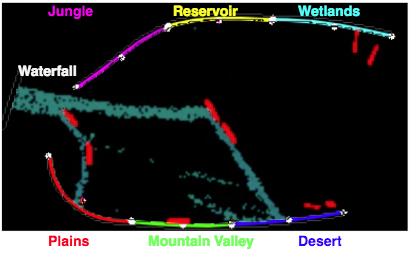
\includegraphics[width=10cm]{connected_worlds_schematic.png}
\caption{Bird's eye view of the CW simulation. Biomes are labeled on the perimeter and logs appear as thick red lines. Water enters via the waterfall and in this image it is mainly flowing from left to right toward the Desert and the Plains.}
\label{fig:connected_worlds_graphic}
\end{figure}




\subsection{Water Cycle}
Every biome in CW shares the common water resource. The amount of water for a given simulation is pre-defined, thus it forms a \textit{limited resource} that students are required to manage carefully. CW simulates a water cycle where water is directed to biomes and used to sustain plants and animals. Evaporation, dependent on the numbers and levels of plants, and rainfall, dependent on the amount of evaporation, brings the water back to the water sources where it once again becomes a usable resource.

\begin{figure}
\centering
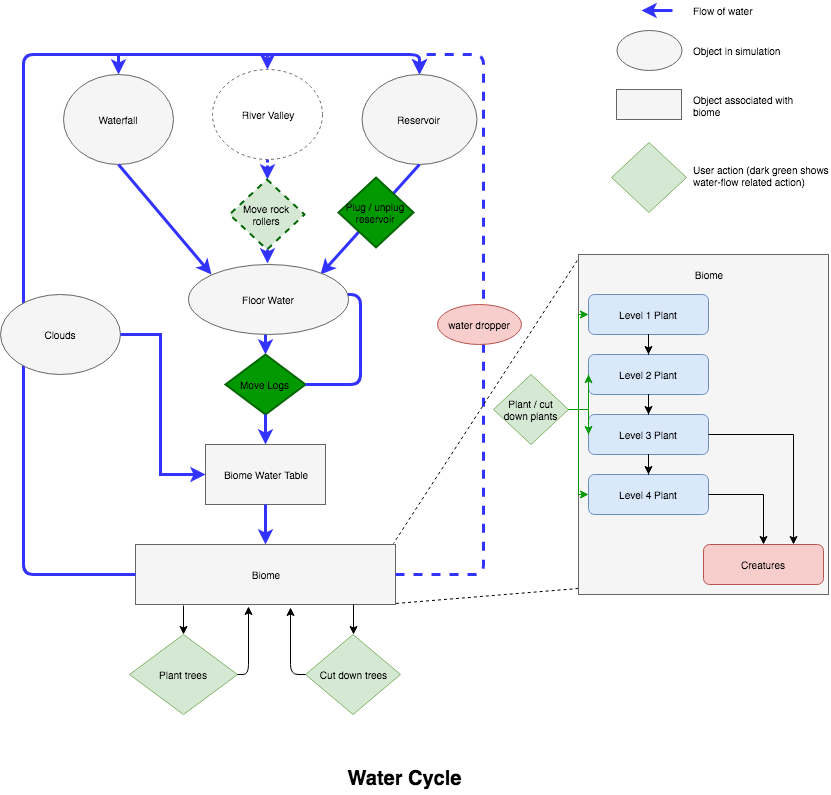
\includegraphics[width=\textwidth]{system_overview_water.png}
\caption{Flow chart showing the water cycles that are present in CW. Blue solid lines represent main water flows, dotted lines represent other possible flows of water that are often not present or are negligible. Green, diamond boxes represent the actions that the students can take that will change the water cycles that are present. Grey circles are regions of the simulation and grey boxes are specifically one of the four biomes.}
\label{fig:system_overview_water}
\end{figure}

Figure \ref{fig:system_overview_water} displays a schematic of the water cycle that is present in CW. Water is available from three sources: the Waterfall, the Mountain Valley and the Reservoir. The Waterfall flows whenever water is available and thus the amount of input water from the Waterfall is out of the students' control. The Mountain Valley is a secondary source of water and it only flows when it rains in this area\footnote{System parameters allow the rain in the Mountain Valley to be turned off, stopping the flow from this area. The rain in the Mountain Valley has been disabled for the experiments presented in this study}. Students choose when to release water from the Reservoir and thus, apart from overflow events, this source of water is directly under their control. Overflow events result when it rains in the Reservoir and the water `spills' out onto the simulation floor when the Reservoir is at full capacity. Students position the logs on the floor of the simulation (see Figure~\ref{fig:connected_worlds_graphic}) to direct some portion of water to some subset of the four biomes. Once a biome has water, the students are able to plant trees. Higher level trees require the presence of lower level trees. The number and level of trees affects the amount of water that the biome requires. Lastly, when water is present in a biome, students can pipe water out of the biome by placing a log at that biome's wall (one of the purple, aqua, red or blue lines in Figure~\ref{fig:connected_worlds_graphic}).



\subsection{Plant-Animal Relations}

Students plant trees and observe the arrival of animals that use the trees to support their habitat. Mimicking a real-world scenario, the fauna for a biome depends on the flora, and the flora are unique for a specific biome. In other words, each biome can support different plants and each type of plant attracts a certain type of animal. Larger and higher level plants require the presence of smaller and lower level plants. Often the animals that are supported by the top level (level 4) plants are the most aesthetically pleasing, and part of the goal for a given simulation might be to attract these animals. Students are thus required to manage their resources to support lower level plants and animals before achieving the top level in a specific biome. The plant and animal relationships are summarized in Figure~\ref{fig:system_overview_plant_animal}.

\begin{figure}
\centering
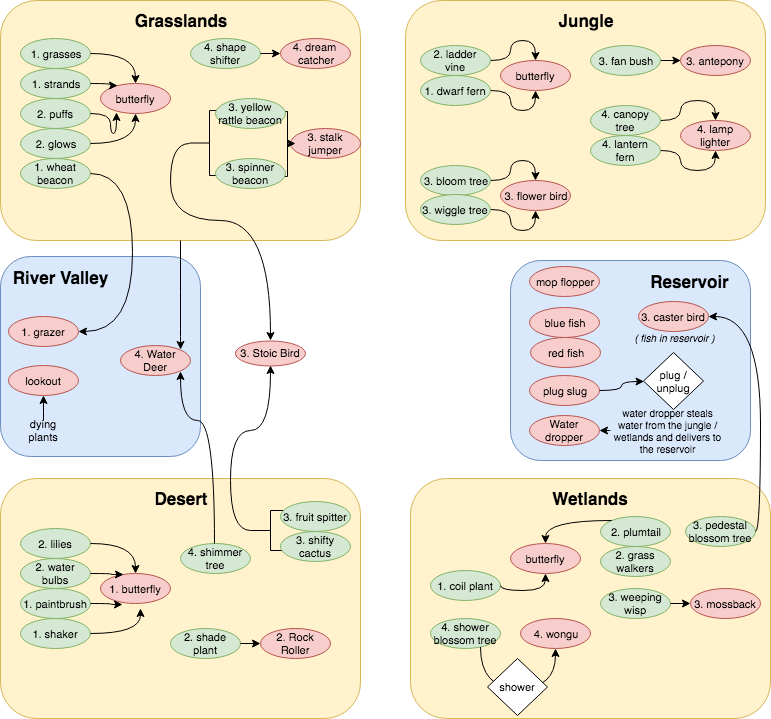
\includegraphics[width=\textwidth]{system_overview_plant_animal.png}
\caption{Map of the relationships between plants, animals and biomes in the CW environment. The biomes are shown in yellow. The blue boxes correspond to areas of the simulation that do support animals but do not have plants that grow there. The fauna-flora specific relations can clearly be seen by the arrows that link the plants (green ovals) and animals (red ovals). The plants and animals are endemic to their biome.}
\label{fig:system_overview_plant_animal}
\end{figure}

\section{Need for Assistive Technology}
The nature of the simulation is complex on a variety of dimensions. The simulation involves a large number of students simultaneously executing actions that change the state of the simulated environment.  No one person - including the teacher or interpreter - can possibly follow what happens, even in a relatively short simulation. Each participant may have a different view of what transpired, depending on the actions he or she took and the state changes that resulted. We propose that it is important to develop tools that can support teachers' understanding of the effects of students' interactions in complex exploratory learning environments such as CW. We introduce a technique for decomposing a complex session into shorter periods where the dynamics of the simulation are stable. Our hypothesis is that these smaller periods will individually be more interpretable than the session as a whole and they will eventually form a subset of useful information that a teacher can draw on when leading a review of the session with groups of students.




\chapter{The Switching State Space Model}\label{ch:2}
\section{Switch Based Models}
The switching state-space Model (SSSM)~\citep{ghahramani2000variational}, or switching linear dynamical system (SLDS)~\citep{fox2009nonparametric}, captures nonlinear dynamical phenomena by allowing discrete points in time where a system switches among conditionally linear dynamical modes. Our primary reason for exploring this model is to perform inference over the assignment of data to specific linear dynamical modes (or regimes), thereby characterizing periods that exhibit dynamics controlled by the regimes. The ease of interpretability of the conditionally linear regimes is an attractive merit of this model, yet the presence of the discrete switch points allows the model to capture a wide variety of non-linear dynamics.

The SSSM has been used for prediction tasks~\citep{fox2007hierarchical,li2003survey} but also for inference tasks~\citep{fox2009nonparametric,jonsen2007identifying,pavlovic2001learning} where the primary goal was to discover latent structure in time series data. \citet{oh2008learning} use the term `learning' to describe the segmentation of the motion of honey bees into different behavioral regimes. They describe the identification of the parameters that characterize the motion within a regime as `quantification'. Similarly, we aim to (1) `learn' the \textit{periods} that define salient regimes in the CW simulation and (2) `quantify' these regimes for the purpose of generating a useful description of the system dynamics.

This work is broadly related to the field of mining information from time series data~\citep{esling2012time,horst2004data}. In contrast to the switching systems that we discuss, other approaches have aimed to cluster short segments from time series data to identify certain patterns that might arise in a database~\citep{vlachos2003wavelet,tanaka2005discovery,patel2002mining}. This involves windowing a time series and defining wavelets, motifs~\citep{patel2002mining} or segments that are commonly found throughout the database. \cite{preston2009event} propose an approach to define and mine for events in a time series database. These previous approaches are concerned with finding small sections or events that might be of relevance within the larger time series. We rather focus on decomposing the \textit{entire} time series into periods that are coherent to a human observer.

\citet{ghahramani2000variational} introduce and give a detailed presentation of the SSSM. \citet{pavlovic2001learning} and \citet{giordani2007unified} use switching models to capture non-linear behavior in a time series, applied to model human motion and econometrics respectively. SSSMs have also been applied in object tracking domains where it is necessary to predict the trajectory of multiple objects~\citep{fox2007hierarchical}. \citet{whiteley2010efficient} introduce a sequential Monte Carlo algorithm for inference over SSSMs using discrete particle filters. We present a new avenue of study in which SSSMs are used to describe complex time series in a way that can be easily interpreted by people and we propose an algorithm to perform posterior inference over the latent variables in this model.

Before describing the SSSM in Section~\ref{sec:switching_state_space_models}, we first provide a brief introduction to the linear state-space model for \textit{continuous} time series data and the hidden Markov model for \textit{discrete} time series data. The SSSM couples these two models and thus this background work is a necessary step towards constructing the SSSM.


\section{Background Information}
\subsection{State Space Models and Hidden Markov Models}\label{sec:state_space_and_hidden_markov_models}
Hidden Markov models (HMM) and state-space models (SSM) define a joint probability density over a sequential collection of hidden state ($\mathbf{X}$) and observed ($\mathbf{y}$) random vectors~\citep{ghahramani2001introduction,shumway2000time}. The HMM refers to the case when the states and observations have discrete values. For example at a time step $t$ the hidden state $\mathbf{X_t}$ is represented by a categorical variable that can take one of $M$ possible discrete values, where a value indexes a state. The associated observations $\mathbf{y_t}$ are discrete symbols where the observation probabilities $P(\mathbf{y_t} \mid \mathbf{X_t})$ can be fully specified by an $M \times K$ observation matrix, with $K$ being the number of possible observation states. Given the hidden state at time $t$ in an HMM, the associated observation is independent of all other observations. Moreover, the hidden states obey the Markov independence property: state $\mathbf{X_{t}}$ is conditionally independent from the previous states ($\mathbf{X_{k}}$ for $k \in 1,2, \hdots, t-2$) and future states ($\mathbf{X_{k}}$ for $k \in t+2, \hdots, T$) given the value of state $\mathbf{X_{t-1}}$ and $\mathbf{X_{t+1}}$ respectively. The joint probability for the sequence of states and observations can be factored as\footnote{Here we use the notation $X_{1:t}$ to refer to all states $X_k, k \in [1,2,\hdots,t]$}:

\begin{equation}\label{eq:joint_prob_ssm}
  P(\mathbf{X_{1:T}}, \mathbf{y_{1:T}}) = P(\mathbf{X_1})P(\mathbf{y_1} \mid \mathbf{X_1}) \prod\limits_{t=2}^{T} P(\mathbf{X_t} \mid \mathbf{X_{t-1}} ) P( \mathbf{y_t} \mid \mathbf{X_{t}} )
\end{equation}

When the model is changed to allow for real-valued state and observation vectors, it is termed a state-space model. The simplest and most commonly used models that follow this structure assume that the transition and output functions are linear and time invariant and the distributions of the state and observation variables follow multivariate Gaussian distributions~\citep{ghahramani2000variational}. The linear Gaussian SSM is defined by the tuple $(A, C, Q, R)$ in:
\begin{equation}\label{eq:hmm_first_order}
  \begin{split}
      \mathbf{X_t} &= A\mathbf{X_{t-1}} + w_t \\
      \mathbf{y_t} &= C\mathbf{X_t} + v_t
  \end{split}
\end{equation}
where $A$ is the state transition matrix, $w_t \sim \mathcal{N}(0,Q)$ is the state transition noise, $C$ is the output matrix and $v_t \sim \mathcal{N}(0,R)$ is the observation noise.

The problem of inference or state estimation for a SSM with known parameters consists of estimating the posterior probabilities of the hidden variables given a sequence of observed values. This inference problem can be broken into \textit{filtering}, \textit{smoothing} and \textit{prediction}~\citep{shumway2000time}. The goal of filtering is to use all the data up to time $t$ to calculate the probability of the hidden state $X_t$. Smoothing, aims to use all of the data available from time $1 \hdots T$ (with $T > t$) to calculate the probability of $X_t$. Lastly, prediction is calculating the probability of the future states $X_{t+1}$ given all the data from time $1 \hdots t$. A minor terminology note is that when we perform filtering and smoothing in the context of linear Gaussian state space models, the algorithms are termed Kalman filtering and smoothing respectively.

\subsection{Forward Algorithm}
The forward algorithm, also termed filtering, aims to calculate the probability that a certain state $X_t$ adopts a specific value using only data that is available up to that point in time ($y_{1:t}$). The joint probability of the latent state and the previous data is:

\begin{equation}\label{eq:fwd_filter}
  \begin{split}
    P(X_t, y_{1:t}) &= \sum_{X_{t-1}} P(X_t, X_{t-1}, y_{1:t}) \\&= P(y_{t} \mid X_t) \sum_{X_{t-1}} P(X_t \mid X_{t-1})P(X_{t-1}, y_{1:t-1})
  \end{split}
\end{equation}

We have applied the Markov independence property where: 
\begin{equation}
	\begin{split}
	y_{t}~\mid~X_t &~\indep~y_{1:t-1},~X_{1:t-1} \\
    X_{t}~\mid~X_{t-1} &~\indep~y_{1:t-1},~X_{1:t-2}
    \end{split}
\end{equation}

Note that the joint probability $P(X_{t-1}, y_{1:t-1})$ can be expressed in the same form as equation~\ref{eq:fwd_filter} but dependent on $P(X_{t-2}, y_{1:t-2})$. This defines an efficient recursive routine for calculating the probabilities for all states up to time $t$ using the past data $y_{1:t}$. Note that $P(y_{t} \mid X_t)$ and $P(X_t \mid X_{t-1})$ are given by the transition and emission probabilities (or the emission likelihood in the SSM) and this recursion can be efficiently implemented using a dynamic programming implementation.

\subsection{Backward Algorithm}
It is not always the case that we need to analyze time series data in a streaming fashion (i.e. where data arrive in real time and we only use past and present data to make state estimation inference). When the data are available in an off-line setting, it is advantageous to use \textit{future} values to help calculate the probability of the state at time $t$. The backward algorithm, also termed smoothing, achieves this by calculating the probability of $X_t$ by using all available data $y_{1:T}$, with $t < T$. The backward recursion depends on the value of the forward filter and a new term that can be factored similarly to equation~\ref{eq:fwd_filter}.

\begin{equation}\label{eq:bkwd_filter1}
  \begin{split}
    P(X_t, y_{1:T}) &= P(y_{1:t}, y_{t+1:T}, X_t) =  P(y_{1:t}, y_{t+1:T} \mid X_t)P(X_t)\\ &= P(y_{t+1:T} \mid X_t)[P(y_{1:t} \mid X_t)P(X_t)]
  \end{split}
\end{equation}

$P(y_{t+1:T} \mid X_t)$ corresponds to calculating the probability of observing the future data given the current state (called backward values). $P(y_{1:t} \mid X_t)P(X_t) = P(y_{1:t}, X_t)$ is the probability from the forward algorithm in equation~\ref{eq:fwd_filter}. We are now able to factor the backward term, again using the Markov independence property:

\begin{equation}\label{eq:bkwd_filter2}
  \begin{split}
    P(y_{t+1:T} \mid X_t) &= \sum_{X_{t+1}} P(y_{t+1:T}, X_{t+1} \mid X_t) \\&= \sum_{X_{t+1}} P(y_{t+1:T} \mid X_{t+1})P(X_{t+1} | X_{t})
  \end{split}
\end{equation}

We can calculate $P(y_{t:T} \mid X_{t})$ in terms of $P(y_{t+1:T} \mid X_{t+1})$ thereby defining the set of backward recursions that are needed to calculate fully the joint probability in equation~\ref{eq:bkwd_filter1}. This recursion is given by:
\begin{equation}\label{eq:bkwd_filter3}
  \begin{split}
    P(y_{t:T} \mid X_t) &= \sum_{X_{t+1}} P(y_t, y_{t+1:T}, X_{t+1} \mid X_t) \\&= P(y_t \mid X_t) \sum_{X_{t+1}} P( y_{t+1:T} \mid X_{t+1} ) P( X_{t+1} \mid X_t )
  \end{split}
\end{equation}

One would therefore start the backward recursion from time $T$ to calculate successively the joint probabilities of the states $X_{t:T}$. From equation~\ref{eq:bkwd_filter1}, it can be seen that the forward and backward recursions are both used to calculate the probability of $X_{t}$ given all of the data $y_{1:T}$. In practice, the forward algorithm is run for one pass of the data from $t=1$ to $t=T$ and then the backward algorithm is run from $t=T$ to $t=1$. Note that we have referred to the HMM in the above equations (the marginalizing steps are summations) but appropriate adjustments (to integrals) will present the SSM filtering and smoothing recursions.

\subsection{Viterbi Algorithm}\label{sec:viterbi_algorithm}
The Viterbi algorithm~\citep{forney1973viterbi} for HMMs recursively finds the most probable path of states that generated the observed data~\citep{nasrabadi2007pattern}. We first define the partial probability $\pi_{t,i}$ to be the probability of the best path for states $X_{1:t}$ that leads to state $X_t = i$ as the terminating state. Intuitively, the best path leading to state $X_t = i$ at time step $t$ must include the best path to $X_{t-1}$ (assuming the same ending state $i$). We can therefore expect a recursive structure to an algorithm that decodes the best state sequences. In the following, we denote $X_i$ as all possible terminating states that can be adopted at the time step $t$.
\begin{equation}\label{eq:viterbi}
  \pi_{t,i} = \max\limits_{\forall X_i} \left\{ \pi_{t-1,j} P(y_t \mid X_i)P(X_i \mid X_{t-1}) \right\}
\end{equation}

The algorithm uses the maximum probability from the previous state along with the observation probabilities for decoding the most likely present state.



\section{Switching State Space Models}\label{sec:switching_state_space_models}
A SSSM includes $M$ latent continuous state-space models and a discrete switching variable. Each of the models, referred to as a regime, has its own dynamics. At each point in time, the switching variable selects one of the individual state-space models to generate an observation vector.

The SSSM model is formalized as:
\begin{equation}
  \begin{split}
      \mathbf{X^{(m)}_t} &= \Phi^{(m)}\mathbf{X}^{(m)}_{t-1} + w^{(m)}_t \\
      \mathbf{Y_t} &= S_t A^{(m)}\mathbf{X}^{(m)}_t + v_t
  \end{split}\label{eq:switching_state_space}
\end{equation}

Here, $X_t^{(m)}$ denotes the latent continuous valued state for process $m$ at time $t$. $S_t$ is a discrete valued switching variable that selects the $m^{th}$ regime such that regime $m$ at time $t$ is active. The real-valued state $X_t^{(m)}$ and the parameters associated with the $m^{th}$ regime produce the real-valued observation vector $Y_t$. The states' evolution over time depends on the regime dependent transition matrix $\Phi^{(m)}$ and the regime dependent noise $w_t^{(m)}$. When the states and observations are assumed to follow Gaussian distributions, each regime can be viewed as a linear Gaussian SSM as discussed in section~\ref{sec:state_space_and_hidden_markov_models}.

Figure \ref{fig:switching_ssm} presents a graphical representation of a SSSM. Edges between nodes represent conditional dependencies, gray nodes are observed variables and white nodes are latent variables. Not shown in the figure are the regime dependent transition noise $w_t^{(m)}$ and the observation noise $v_t$ which have the same interpretation as the noise models in the SSM. $A^{(m)}$ is the output matrix in the state space formulation, which can be regime dependent but for the applications that follow, it is taken to be the identity matrix.

\begin{figure}
  \centering
  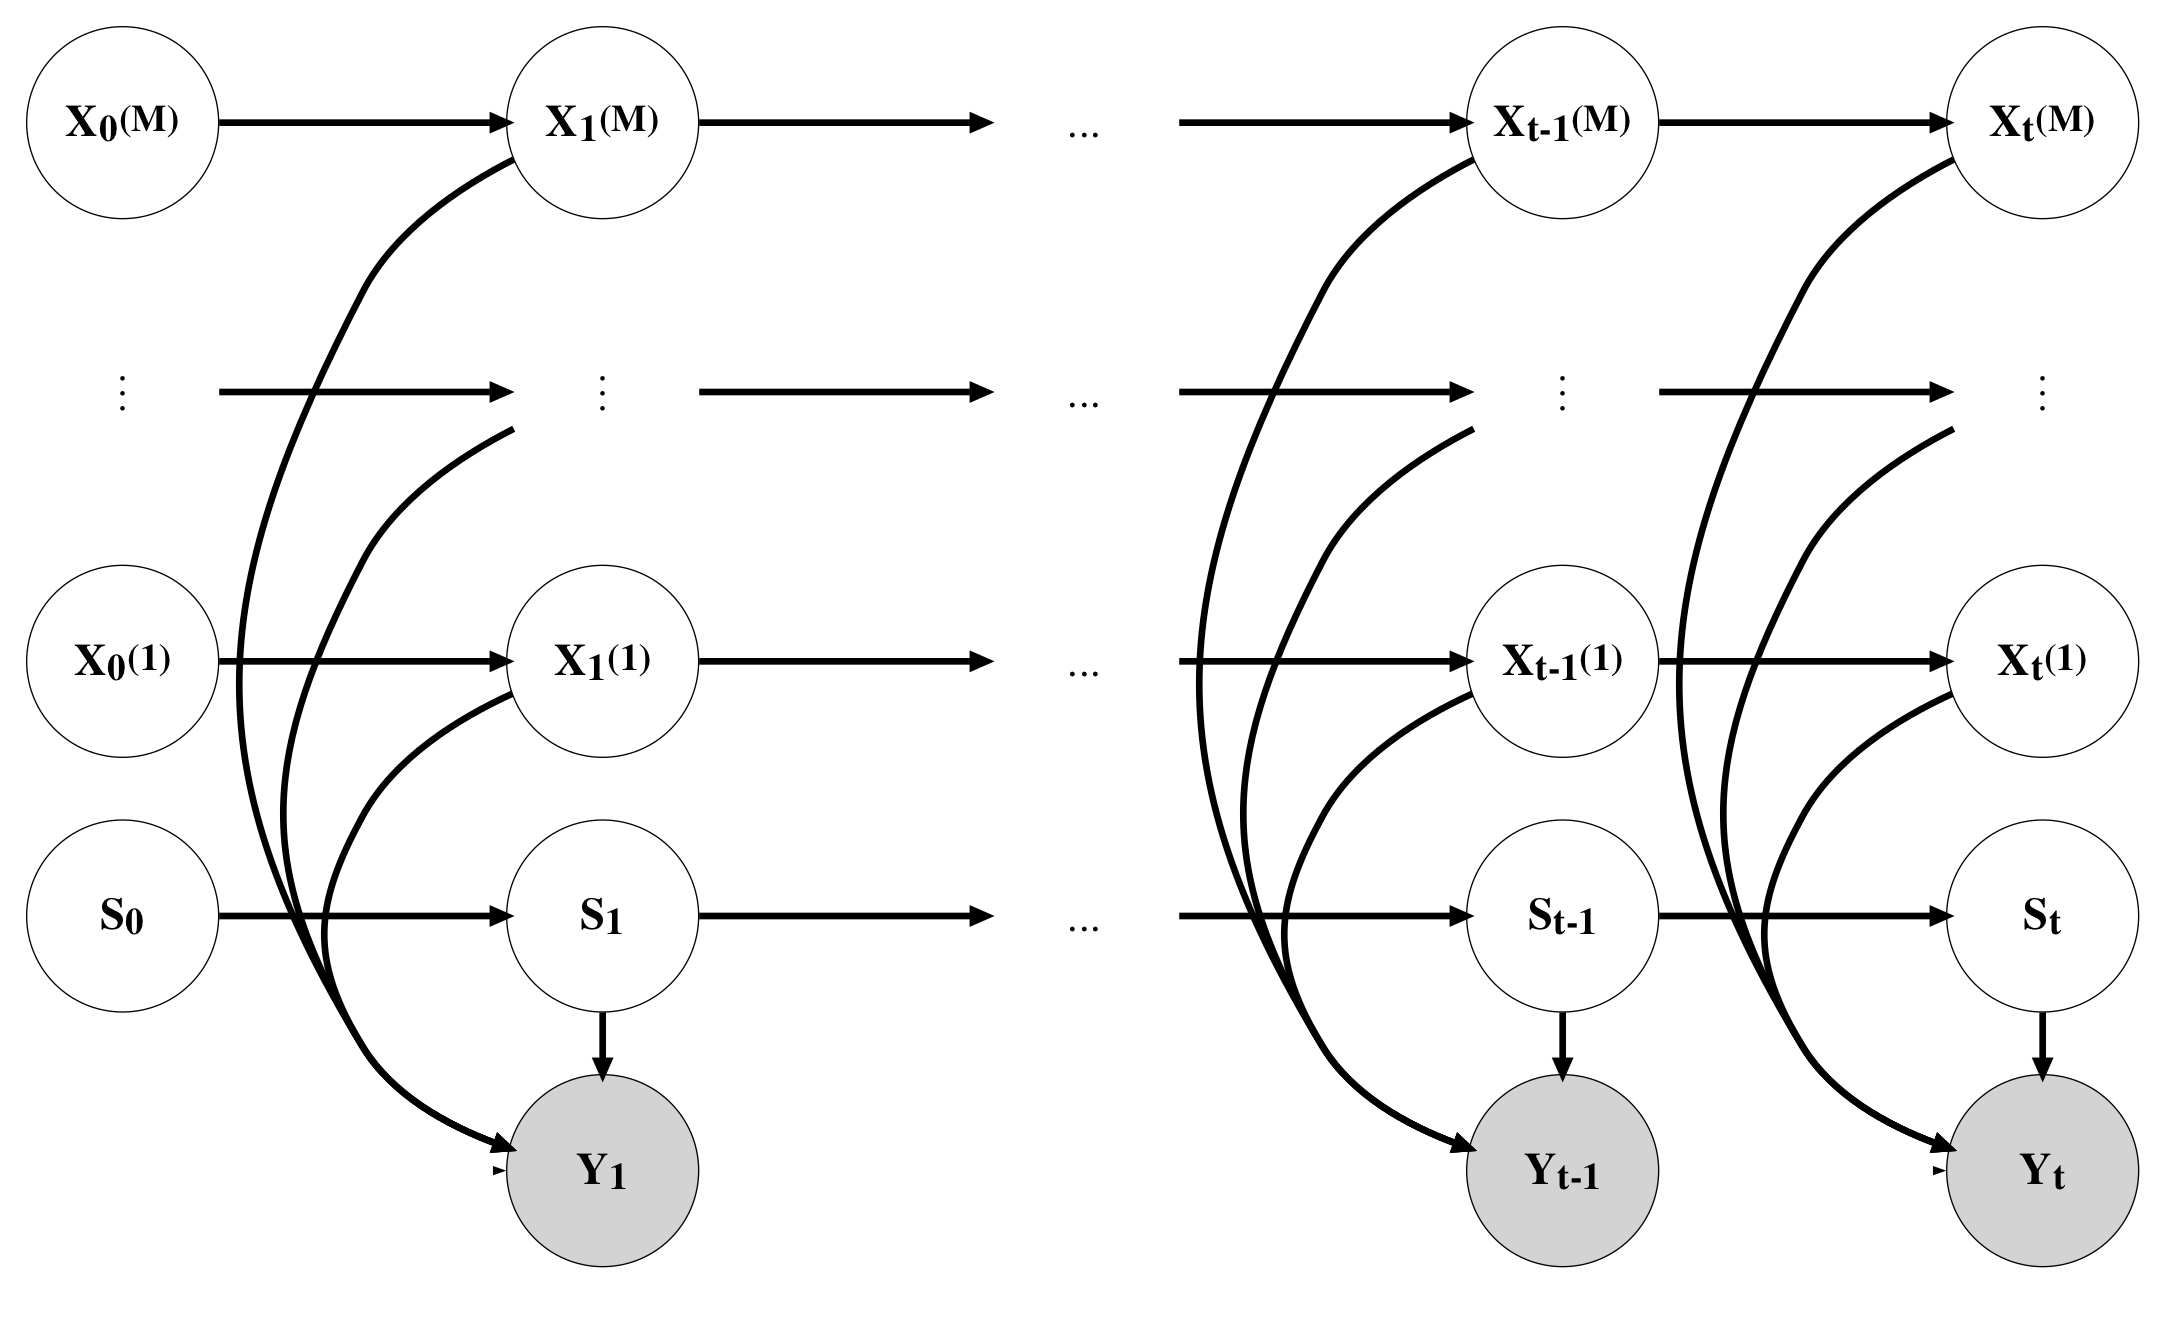
\includegraphics[width=12cm]{switching_ssm.png}
  \caption{Graphical model for the switching-state space model. A latent discrete switching variable ($S_t$) selects an active, real-valued state space model ($X^{(m)}_t$). The observation vector ($Y_t$)  depends on the active regime at time $t$.}
  \label{fig:switching_ssm}
\end{figure}

\subsection{Interpretability of the SSSM}\label{sec:interpretability_of_ssm}
We illustrate the SSSM interpretability by presenting an example of how it can describe the effects of students' interactions in CW. $Y_t$ represents the observed water level in the different areas of the simulation at time $t$. $X_t^{(m)}$ describes the expected levels of water under regime $m$ at time $t$. $\Phi^{(m)}$ controls the water flow in the simulation according to the transitions in regime $m$. $S_t$ selects which of the regimes to use to describe the water levels $Y_t$.

A single regime is insufficient for modeling the effects of students' interactions with CW. This is because students' actions have complex effects on the system dynamics. For example when students choose to direct water to the Desert and Plains and plant many trees in the Desert, the system dynamics are entirely different to the case when water is directed towards the Jungle and the Desert and the Plains are left to dry. We therefore need to define multiple regimes, where each regime describes a series of events that can be (stochastically) explained by the regime dynamics. A regime is active for a duration of time in CW. This duration is called a period. In our example, in one period, water is mainly flowing to the Plains and to the Desert. In the next period, students move the logs to re-route water flow to the Jungle (potentially because plant life is dying). The students may also release water from the Reservoir to direct that to the Desert. These dynamics will be captured by the second period's regime parameters. The output of the model is a number of regimes (that are active for the corresponding periods) that together capture the system dynamics, but individually can be easily interpreted.

Note that we have described a system where the direct observation of the underlying process is available. This is termed a vector autoregressive model (VAR) with switching~\citep{fox2009nonparametric, shumway2000time,kim1994dynamic}. An order $r$ VAR process with observations $\mathbf{y_t}$ is defined by:
\begin{equation}\label{eq:var}
  \mathbf{y_t} = \sum\limits_{i=1}^{r} A^{(m)}y_{t-i} + w^{(m)}_t \hspace{20pt} w^{(m)}_t \sim \mathcal{N}(0, Q^{(m)})
\end{equation}

Equation~\ref{eq:var} shows that the observations at time $t$ depend linearly on the previous $r$ observation vectors. In CW, we use a $VAR(1)$ process. Since the SSSM generalizes the switching $VAR$ process, we refer to the SSSM throughout this study but recognize that the models also apply to the VAR specific case. Any $VAR(r)$ process can be written in a SSM format as follows:

\begin{equation}\label{eq:ssm_rep_of_var_state}
  \mathbf{X_t} =
  \begin{bmatrix}
      A_{1}       & A_{2} &  \dots & A_{r} \\
      I           & 0     &  \dots & 0 \\
      \vdots      & \ddots&  \vdots& \vdots \\
      0           & \hdots&   I    & 0
    \end{bmatrix} \mathbf{X_{t-1}} +
  \begin{bmatrix}
    I \\
    0 \\
    \vdots \\
    0
  \end{bmatrix} w^{(m)}_t
\end{equation}

\begin{equation}\label{eq:ssm_rep_of_var_output}
  \mathbf{y_t} = \begin{bmatrix} I & 0 & \hdots & 0 \end{bmatrix} \mathbf{X_t}
\end{equation}

It is worth highlighting that for the SSSM in general, and indeed for the inference that we target in CW, the model is highly under-specified. The points in time that define the changes between regimes are unknown, the duration of the periods are unknown and the regime specific parameters are unknown. Moreover, the number of regimes is unknown. The goal of Section~\ref{sec:posterior_inference_sssm} is to introduce an efficient unsupervised algorithm for performing inference over these unknown variables. For this implementation, we define a reasonable number of regimes $M$ but in Section~\ref{sec:non-parameteric} we discuss the related work in Bayesian non-parametrics which allow us to remain agnostic about the number of regimes that are present.


\section{Inference in Switching State Space Models}\label{sec:inference_for_sssm}
We aim to perform inference over the latent states $X_t^{(m)}$, the regime parameters $\Phi^{(m)}$, and latent switching variable $S_t$ in the SSSM defined in equation~\ref{eq:switching_state_space}. Computing posterior distributions for SSSMs is computationally intractable~\citep{murphy2002dynamic, kim1994dynamic}. To illustrate, in Figure~\ref{fig:switching_ssm} note that the graph consists of $M$ state space models that are marginally independent. These models become conditionally dependent when $Y_t$ is observed (as is the case in this graph). The result is that $X_t^{(m)}$ is conditionally dependent on the value of all of the other latent states and switching variables for times $1$~through~$T$ and regimes $1$~through~$M$~\citep{murphy2002dynamic,ghahramani2000variational}.

Due to the intractability, previous approaches use approximation methods such as variational inference~\citep{ghahramani2000variational} or a `merging of Gaussians'~\citep{kim1999state,murphy2002dynamic} to address the inference problem. Variational inference approximations transform an intractable Bayesian expectation problem into an optimization problem by minimizing the Kullback-Leibler divergence between a simpler family of approximating distributions and the unknown, intractable posterior~\citep{attias2000variational,saul1996exploiting,saul1996mean,blei2003latent}. The merging of Gaussians uses a single Gaussian to approximate the mixture of $M$ Gaussians at each time step. While these methods have seen success in previous examples, they cannot be applied to our domain. This is because they allow the system to move back and forth between regimes, resulting in frequent regime changes that can hinder the interpretability of the model. This work takes a different approach by imposing structure on the model to address both inference and interpretability challenges. Another avenue for inference is the sticky hierarchical Dirichlet process hidden Markov model (sticky HDP-HMM)~\citep{fox2009nonparametric,fox2007hierarchical}, an extension of the hierarchical Dirichlet process (HDP)~\citep{teh2005sharing}, that relaxes the within-cluster exchangeability assumption of the HDP. We discuss this model in further detail in Section~\ref{sec:non-parameteric} and present it as a promising avenue for future work.

To perform inference over the regime parameters and the switch assignments, we make two assumptions, which arise from the need to create human interpretable descriptions of the complex system behavior. \textbf{Assumption 1:} the system advances through a series of regimes, each regime is active for a period, and then switches to an entirely new regime, one that has not been used before. \textbf{Assumption 2:} the regime remains active for the maximum possible time for which it can be used to describe the period.

Without making these assumptions there are $M$ possible assignments of regimes for each time step, making a total of $M^T$ combinations of possible assignments, which is exponential in the number of time steps. Moreover, in the worst case, the number of possible periods is bounded by $T$ with a switch at every time step. In contrast, under our assumptions, there are only two possible assignments of regimes for each time step (i.e., the choice is to stay in the current regime or to progress to the next regime), making for a total of $2^M$ combinations of possible assignments, where $M$ is constant.  The number of possible periods under this methodology is bounded by $M$.
% We further hypothesize that the forced reduction in complexity of the fitted model would significantly simplify the interpretability of the model for a human.

\subsection{Approximate Maximum Likelihood Estimation for Switching State Space Models}\label{sec:gaussian_merging}

\cite{shumway1991dynamic} assume known regime parameters and use the state space specific observation probabilities to perform inference over the switching variables in the SSSM (using the Viterbi algorithm presented in \ref{sec:viterbi_algorithm}). Their implementation is extended by \cite{kim1994dynamic, kim1999state} and \cite{bar1993estimation} to handle the case where the regime parameters are unknown. The maximum likelihood estimate (MLE) presented by these authors employs a `Gaussian merging' assumption~\citep{ghahramani2000variational} to make the inference tractable. \cite{kim1994dynamic} presents a basic filtering and smoothing algorithm for the SSSM, combined with a MLE of the unknown regime parameters.

In the standard state space filtering formulation, we wish to calculate the expected value of the latent states $X_t$, given the observations $y_{1:t}$. This corresponds to calculating:
\begin{equation}\label{eq:kim_ssm_expected_val}
  X_{t \mid t} = E[X_t \mid y_{1:t}]
\end{equation}
Following state space notation for the expectation, $X_{t \mid t}$ refers to the expected value of the latent state at time $t$ given the previous observations. Similarly, $P_{t \mid t}$ refers to the covariance of the estimate for $X_{t \mid t}$ conditioned on the data $y_{1:t}$:
\begin{equation}\label{eq:kim_ssm_covariance}
  P_{t \mid t} = E[(X_t - X_{t \mid t})(X_t - X_{t \mid t})' \mid y_{1:t}]
\end{equation}
With the introduction of the switching variable $S_t$, we require $X_{t \mid t}^{(i,j)}$ which is the expected value for $X_t$, conditioned on the past data $y_{1:t}$ and the value of $S_t = j$ and $S_{t-1} = i$. The expected values for the state and the covariances associated with these estimators are:

\begin{equation}\label{eq:kim_sssm_expected_val}
	\begin{split}
  X_{t \mid t}^{(i,j)} &= E[X_t \mid y_{1:t}, S_{t-1} = i, S_t = j] \\
  P_{t \mid t}^{(i,j)} &= E[(X_t - X_{t \mid t})(X_t - X_{t \mid t})' \mid y_{1:t}, S_{t-1} = i, S_t = j]
  	\end{split}
\end{equation}

In computing the Viterbi algorithm, we would require the expectations and covariances in equations~\ref{eq:kim_sssm_expected_val} for every possible value for $i$ and $j$. If there are $M$ regimes in the model, this results in $M^2$ terms that are calculated at every time step. The resulting Kalman filter experiences a growth of terms that is exponential in $T$, a problem that is also encountered in Section~\ref{sec:posterior_inference_sssm}. \cite{kim1994dynamic} proposes an algorithm for reducing the $(M \times M)$ posteriors for $X_{t \mid t}^{(i,j)}$ into just $M$ posteriors by merging the Kalman filter to a single posterior at each time step.

The approximation that \cite{kim1994dynamic} employs is given by:
\begin{equation}\label{eq:collapsed_likelihood}
  X_{t \mid t}^{(j)} = \frac{\sum\limits_{i=1}^{M} P[S_{t-1}=i, S_t=j \mid y_{1:t}]X_{t \mid t}^{(i,j)}}{P[S_t = j \mid y_{1:t}]}
\end{equation}
\cite{ghahramani2000variational} call this the `Gaussian merging' approach because in equation~\ref{eq:collapsed_likelihood}, $X_{t \mid t}^{(j)}$ represents the re-normalized mixture of Gaussians in the numerator. $X_{t \mid t}^{(j)}$ represents the $E[X_t \mid S_t = j, y_{1:t}]$ with the $S_t = i$ dependency marginalized out. The covariance of this estimator $P_{t \mid t}^{(j)}$ is calculated in a similar fashion and can also be interpreted as the posterior from a weighted mixture of normals\footnote{See the derivation in \cite{kim1994dynamic} for further details.}.

Finally, we can use numerical optimization to perform parameter estimation. The Gaussian merging is used to construct a forward filter to approximate the likelihood of the regime parameters and the associated switches. This likelihood is maximized to present an approximate MLE for the parameters. It is worth noting that the optimization is highly susceptible to local maxima due to the tightly coupled nature of the regime parameters and the locations of the switch points. Thus, the numerical optimization might terminate early at these local optima leading to incorrect inferences. This is seen in Section~\ref{sec:experiment1-empirical-validation}.

\subsection{Background on Inference for Probabilistic Models}

\subsubsection{Introduction to Bayesian Inference}

Bayesian models lend themselves to domains where the interpretability of the model is of importance~\citep{gelman2014bayesian}. The model structure that is imposed on a domain is considered part of the prior knowledge and as such, inference about the latent variables has a strong interpretability within the defined model's structure. Bayesian statistics is derived from Bayes rule:

\begin{equation}\label{eq:bayes_rule}
	P(\theta \mid X) = \frac{P(X \mid \theta)P(\theta)}{\int P(X \mid \theta)P(\theta) d\theta}
\end{equation}

The denominator in equation~\ref{eq:bayes_rule} represents the normalizing constant that is not dependent on the parameter vector $\theta$. This integral is often intractable and thus evaluation of the posterior $P(\theta \mid X)$ becomes a challenging objective. Conjugate structure in certain problems allows for the direct computation of an analytical solution for the posterior distribution. This structure is often not available, or conjugacy imposes undesirable restrictions given the problem setting. Thus other means for \textit{approximating} the posterior distribution are required when performing inference in Bayesian models. Variational inference~\citep{attias2000variational,saul1996exploiting,saul1996mean,blei2003latent} is an approach that is commonly used to approximate the posterior distribution. Variational inference can give misleading results when dealing with highly correlated and co-dependent data, such as data present in time series models~\citep{turner2011two}. Monte Carlo (MC) approximations present a different avenue for the approximation of an intractable posterior distribution. MC techniques are appealing due to their strong convergence properties albeit at a high computation cost~\citep{mackay1998introduction}.

MC sampling is a popular approach for performing posterior inference in Bayesian statistics as it presents a technique for evaluating expectations under an unknown target distribution~\citep{mackay1998introduction}. MC techniques use the fact that given independent samples $x^{(r)}$ from a target distribution $P(X)$, the samples can provide a robust estimator of expectations under the distribution defined by $P$. The strong convergence properties of MC methods state that the error of the estimator tends to $0$ as the number of samples tends to $\infty$. Concretely, the expectation $\mathbf{\Phi}$ of a function $\phi$ under the distribution $P$ can be approximated by the MC estimator $\hat{\Phi} = \frac{1}{R}\sum\limits_r \phi(x^{(r)})$. Here $\mathbf{\Phi} = \int P(x)\phi(x) dx$ is the true value for the expectation~\citep{mackay1998introduction}. Examples of MC sampling include rejection, importance and slice sampling~\cite{neal2003slice} but these techniques are shown to scale poorly to high dimensional and tightly correlated distributions.

\subsubsection{Markov Chain Monte Carlo}\label{sec:mcmc}
Rather than attempt to draw entirely independent samples from the target distribution, we can use current samples to propose new, dependent samples in the form of a Markov chain. Given a valid transition function in the Markov chain, the stationary distribution of the samples converge to the true target distribution~\citep{mackay1998introduction}. The subset of MC techniques that use current samples to propose new, dependent samples is termed Markov Chain Monte Carlo (MCMC). When explicit structure of the domain allows the derivation of complete conditionals\footnote{The \textit{complete conditionals} are the conditional distributions of a subset $T \subset \{ 1, 2, \hdots n \}$ of the parameters given all other parameters not in $T$.}~\citep{mackay1998introduction}, Gibbs sampling presents an attractive MCMC technique. More generally, the Metropolis method is used when complete conditionals are not available.

Metropolis is an algorithm for sampling from an unknown distribution with density $\frac{1}{Z} f(x)$. Here, $f(x)$ is an un-normalized probability density and $\frac{1}{Z}$ is the normalizing constant. The algorithm uses the current sample $x$ to propose a new sample $x^*$ from a given proposal distribution (i.e., $g(x^* \mid x)$). The candidate sample $x^*$ is evaluated according to an acceptance probability $a(x^*, x)$, and if the proposal state is accepted, we set the new sample $x' = x^*$. Alternatively, the new sample is set to the previous sample $x' = x$. The acceptance probability for Metropolis is given by:
\begin{equation}
	a(x^*, x) = min \left[ 1, \frac{g(x \mid x^*)}{g(x^* \mid x)} \frac{f(x^*)}{f(x)} \right]
\end{equation}

It has been shown that the update from $x$ to $x'$ leaves $f$ invariant~\citep{mackay1998introduction, gelman2014bayesian} and therefore as the Markov chain is run indefinitely, the Metropolis algorithm provably converges to drawing samples from the stationary distribution that is defined by density $f(x)$. Metropolis provides a general structure for defining a Markov chain that will converge to drawing samples from the target distribution. However, the algorithm is highly dependent on the proposal distribution $g$, and if $g$ is poorly chosen, the algorithm can reject many samples resulting in a slow convergence of the chain. Similarly, a poor choice of $g$ can result in samples that are highly correlated and thus the new samples do not explore the posterior distribution sufficiently for a given \textit{limited number} of samples. Variants of the Metropolis algorithm have been proposed to assist the exploration of the target distribution. The state of the art is the Hamiltonian Monte Carlo (HMC) method and the No U-Turn Sampler (NUTS) which modifies HMC by tuning parameters automatically.

\subsubsection{Hamiltonian Monte Carlo and the No U-Turn Sampler}\label{sec:hmc_nuts}

Hamiltonian Monte Carlo~\citep{neal2011mcmc} was introduced as another MCMC technique to combat the inadequacies of Metropolis. In particular, HMC introduces \textit{a structured and deterministic} search of the probability space before making a proposal sample. The aim of HMC is to efficiently \textit{explore} the target distribution and thus draw pseudo-independent samples while still using the convergence guarantees of MCMC.

HMC is inspired by statistical mechanics where particles in space are known to interact and follow trajectories that are defined by Hamiltonian mechanics~\citep{neal2011mcmc}. Hamiltonian equations define the energy of the particle over momentum ($p$) and position ($q$) phase space. HMC is an auxiliary model where a momentum variable ($p$) is introduced that allows us to simulate a deterministic dynamic through $(p,q)$ space with the analogy that the probability corresponds to the distribution of the position of a particle. Hamiltonian dynamics have three properties that make this simulation useful for the MCMC use-case. The Hamiltonian (1) preserves energy, (2) has reversible dynamics and (3) conserves volume in phase space. Properties (1) and (3) allow the simulation of Hamiltonian dynamics along some probability distribution contour such that a new proposal is found that has the same energy as the current sample. Property (2) is important for conserving \textit{detailed balance}, a property of MCMC that ensures the target distribution is left invariant by the simulation (i.e., does the sampler actually converge to drawing samples from the target distribution).

For HMC, a numerical integration scheme is needed to simulate the differential equations that are defined by the Hamiltonian~\citep{neal2011mcmc}. This numerical integration scheme is known as a symplectic integrator as is required to conserve energy throughout the course of the simulation, corresponding to maintaining property (1) of the Hamiltonian. The leapfrog method presents a small adjustment to Euler's numerical integration scheme by alternating between the momentum and position updates with a half-step spacing the discretization updates. The integration requires two user-defined parameters: the step size $\epsilon$ and the number of steps used to simulate the dynamics $L$. Tuning $L$ and $\epsilon$ is shown to be challenging in practice and can have dramatic effects on the success of the HMC algorithm for exploring the entire typical set of the target distribution~\citep{hoffman2014no}. Note that choosing $\epsilon$ too small will result in unnecessary computation to simulate Hamiltonian trajectories. Choosing $L$ too large will result in Hamiltonian trajectories returning to their starting point, defeating the goal of exploring the target probability space to find \textit{independent} samples.

\cite{hoffman2014no} introduce the No U-Turn Sampler (NUTS) to automatically tune these two parameters for the given problem. In essence the algorithm constructs a binary tree simulating the HMC dynamics for a number of steps that doubles with each level in the tree. The algorithm terminates when the simulated dynamics experience a momentum that points back toward the starting point of the simulation. The imprecise nature of the numerical integration scheme requires that the proposed state be accepted with an acceptance probability from the Metropolis update\footnote{If the Hamiltonian dynamics were simulated perfectly, there would be no need for this acceptance check. Because there is error in the numerical integration, we need to accept the proposed sample in the same way that Metropolis accepts proposed samples.}. NUTS is implemented in a number of probabilistic programming languages to enable automatic inference in complex user-defined models. We use the Stan-MC\footnote{\url{http://mc-stan.org/}}~\citep{carpenter2016stan} implementation of NUTS for conducting inference in the model defined in Section~\ref{sec:posterior_inference_sssm}.

\subsection{Algorithm for Posterior Inference of Switching State Space Models}\label{sec:posterior_inference_sssm}

\subsubsection{Non-identifiability and Label Switching}
Computing the posterior distributions over the latent variables in an SSSM corresponds to approximating the joint distributions over $X_t^{(m)}$, $S_t$ and $\Phi^{(m)}$, given the observation vector $\mathbf{Y}$. A well known problem with MCMC inference in mixture models is that of identifiability~\citep{jasra2005markov}. Models are non-identifiable when two sets of parameters can explain the observed data equally well. This problem is also referred to as label switching as the labels given to classes are unrelated to the class specific parameters. MCMC samplers experience a random permutation of labels during sampling and the resulting posterior distribution is not class specific but rather multi-modal and identical to the marginal posteriors for the individual classes.

This phenomenon can be seen in a simple Gaussian mixture model with means $\mu_0, \mu_1$ and covariances $\Sigma_0, \Sigma_1$. The marginal posterior distributions of the parameters are identical. Figure~\ref{fig:label_switching_example} presents the posterior sample traces for the means from a one dimensional Gaussian mixture model with true means $\mu_1 = -1, \mu_2=1$ and standard deviations $\sigma_1=\sigma_2=0.75$. The label switch can be clearly seen at samples indexed 1000 and 2000 respectively. The smeared posterior distributions for the mean parameters are also clearly evident. If the chain was not truncated (and if other MCMC chains were run), the posterior distributions for $\mu_0$ and $\mu_1$ would be identical. A solution to the identifiability problem is to add constraints on the model prior (e.g., enforcing $\mu_0 > \mu_1$) which makes the prior not symmetrical. However, defining such constraints in higher-dimensional domains is non-trivial.

\begin{figure}
  \centering
  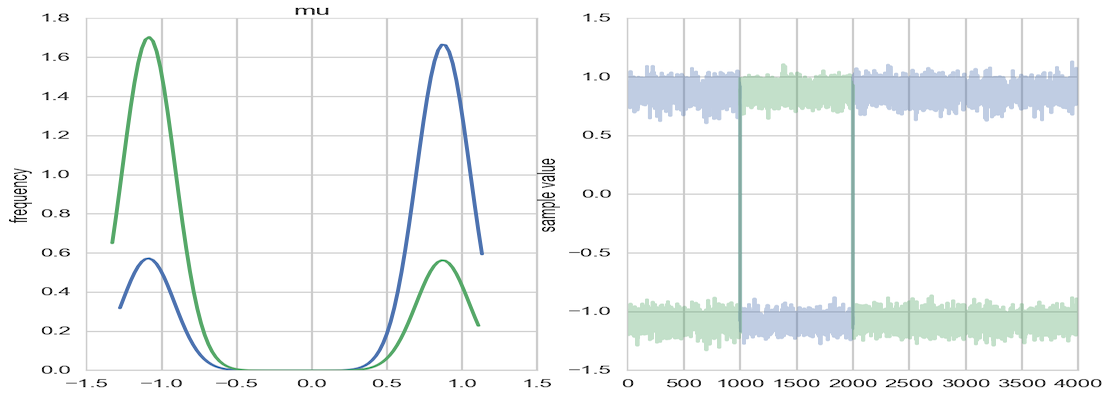
\includegraphics[width=\textwidth]{label_switching_example.png}
  \caption{Posterior samples and associated density plot from the posterior of a Gaussian mixture model with true parameters $\mu_1 = -1, \mu_2=1, \sigma_1=\sigma_2=0.75$. Left shows the density plot for the posterior of the mean parameters. Right shows the posterior sample trace. The label switches can be seen at samples 1000 and 2000 resulting in the multi-modal posterior on the left.}
  \label{fig:label_switching_example}
\end{figure}

Another possible solution for the identifiability problem is to provide labels for part of the data. This is termed semi-supervised learning and we incorporate this solution into our model. In the context of the CW domain, we can label observations as belonging to one regime or another. Let $S_{t, t+1,\ldots, t-1+K,t+K}$ be a consecutive set of $K$ state variables such that $S_t$ and $S_{t+K}$ have known value assignments (regime $m$ and regime $m+1$, respectively). The values for the state variables $S_{t+1,\ldots,t-1+K}$ are unknown. By Assumption 1, the switch between regimes $m$ and $m+1$ occurs at some $S_l$ where $t \leq l \leq t+K$. Therefore, the value of $S_l$ determines the values for all of the unknown states in this period as $S_t$ is assigned to regime $m$ for $t<l$ and it is assigned to regime $m+1$ for $t \geq l$.

\subsubsection{Algorithm Sketch}
We provide a sketch of this process in Algorithm~\ref{alg:constrained_alg}. \textbf{Step 1} initializes the $M$ supervised switch variables, one per regime. The labeled switch variables are spaced uniformly in time and are assigned to regimes in increasing order according to Assumption 1. This uniform method for initialization can be justified  by Assumption 2, in that  any set of regimes  that provides an interpretable model is sufficient. The number of expected  time steps in each period is $K=T/M$, and there are  $K-2$ unlabeled switch variables between each pair of  switch variables assigned to regimes.

\textbf{Step 2} performs MCMC sampling to approximate the posterior of the model. For the case when the value of the switch variable is known, the posterior of $X^{(m)}_t$ can be directly sampled by following the structure of a state space model. In the case where the switch variable is unknown, we have a marginalization problem over the two possible values of $S_t$. For the hidden Markov model (HMM) structure this can be efficiently computed with the forward algorithm~\citep{shumway2000time}. To formulate the HMM forward algorithm, we use the observation probabilities from the individual state space models in place of the emission probabilities of a standard HMM. Here, $\pi_{S_i}$ refers to the belief of the state of the switching variable given the evidence up to that point in time.

\textbf{Step 3} uses the regime specific parameters $\Phi^{(m)}$ to make a maximum a posteriori (MAP) assignment of an observation to a regime using the Viterbi algorithm, thereby specifying the value of $S_t \forall t \in [1:T]$.

\LinesNotNumbered
\begin{algorithm}
\caption{Posterior inference algorithm}\label{alg:constrained_alg}
\textbf{Input: } $M$ (number of regimes), $\mathbf{Y}$ (vector of observations for $T$ time steps).\\
\nextnr
Initialization: Label one datapoint per regime, leaving $T - (M+1)$ unlabeled datapoints.\\
\nextnr
MCMC Inference: Draw samples for $X_{t}^{(m)}$ from the posterior distribution defined by the structured probability model:\\
	\For{$Y_t$ in $\mathbf{Y}$}{
		\eIf{$S_t=m$ is known}{sample from $P(X_{t}^{(m)}, \Phi^{(m)} \mid X_{t-1}, S_t=m, Y_t)$}
        {marginalize over $S_t$. Sample from  $\sum\limits_{i=m-1}^{m} \pi_{S_i}P(X_{t}^{(i)}, \Phi^{(i)} \mid X_{t-1}, S_t=i, Y_t)$}
	}
\nextnr
Posterior Inference: Use the posterior for regime parameters ($\Phi^{(m)}$) to run a Viterbi pass on the data $\mathbf{Y}$ to make a maximum likelihood assignment of the value of $S_t$ to regime $m$ (thereby learning the switching variables $S_t$).\\
\textbf{Output: } $S_t$ (assignments to regimes), $\Phi^{(m)}$ (regime specific posterior distributions).
\end{algorithm}

 Algorithm~\ref{alg:constrained_alg} can be computed on a SSSM where Assumptions 1 and 2 are appropriate. Such a model is shown in Figure~\ref{fig:updated_ssm_graphical_model}. The model depicts a subset of the time series with $K$ time steps from time $t$ to time $t+K$. There are two supervised labels at the boundaries of the subset with the variable $S_t$ assigned to regime $m$ and variable $S_{t+K}$ assigned to regime $m+1$. The unknown $K-2$ states in between are marginalized over such that the regime specific posteriors can still be approximated. This model is repeated for the $M-1$ switches in the data. The setup is flexible in that informative priors for the model noise and transition matrices can be specified (and related) as required by domain knowledge.

\begin{figure}
  \centering
  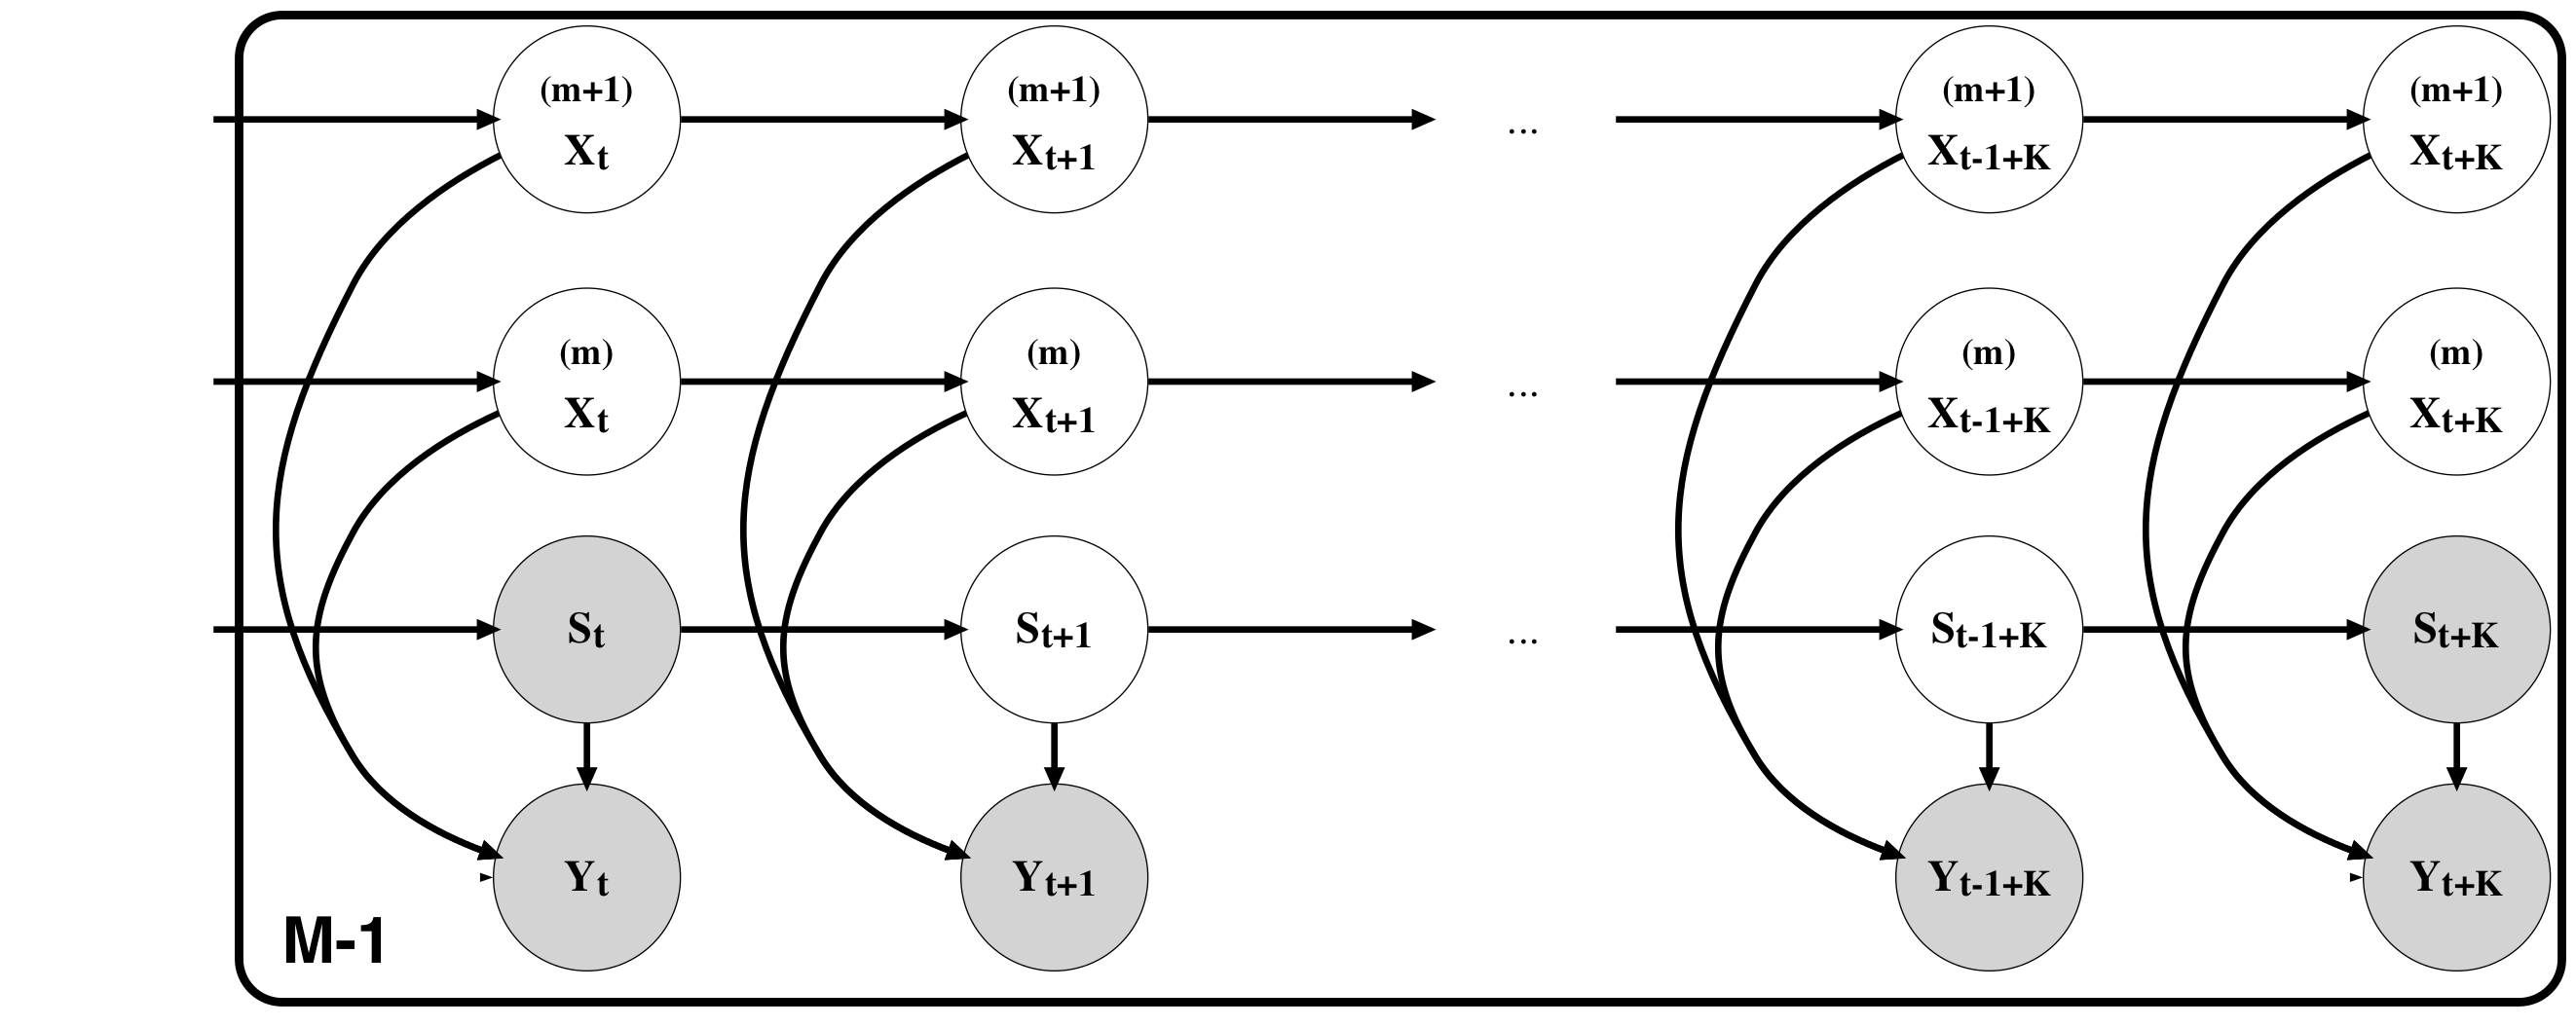
\includegraphics[width=\textwidth]{switching_ssm_constrained.png}
  \caption{Updated graphical model showing the semi-supervised switching labels, along with the choice of only two chains between two semi-supervised points. This representation is repeated $M-1$ times to describe the $M-1$ switches between the $M$ regimes. Note that the labeled switch variables at the boundaries ($S_t$ and $S_{t+K}$) are shared between successive regimes.}
  \label{fig:updated_ssm_graphical_model}
\end{figure}




\chapter{User Study}\label{ch:3}
\section{User Study Empirical Validation}
We evaluate two aspects of Algorithm~\ref{alg:constrained_alg}. First, we show that it finds a good representation for the true change points in a synthetic dataset. Second, we implement two experiments to test whether the inferred periods are interpretable to independent human validators. The first of these experiments aims to verify the salience of the inferred change points within the context of CW. The second experiment is to verify the intelligibility of the automatically generated descriptions for the inferred periods. Due to the tightly coupled relationship between the period boundaries and the regime specific parameters, separating these two factors for comparison is exceedingly difficult. However, between the two experiments, we evaluate the interpretability of the joint inference over the periods and the associated regime parameters. The evaluations suggest that the proposed techniques produce results that do have interpretabilty in the CW domain.

\section{Evaluation on Synthetic Data}

\begin{equation}
  \begin{split}
      \mathbf{X^{(1)}_t} = 0.99 \,\mathbf{X_{t-1}} + w^{(1)}_t \hspace{10pt} & w^{(1)}_t \sim \mathcal{N}(0,1) \\
      \mathbf{X^{(2)}_t} = 0.9 \,\mathbf{X_{t-1}} + w^{(2)}_t \hspace{10pt} & w^{(2)}_t \sim \mathcal{N}(0,10) \\
      \mathbf{Y_t} = S_t\mathbf{X_t} + v_t \hspace{10pt} & v_t \sim \mathcal{N}(0,0.1)
  \end{split}\label{eq:switching_state_space_results}
\end{equation}

Equation~\ref{eq:switching_state_space_results} (an adapted model from \citet{ghahramani2000variational} where the state space is disjoint at regime switches) describes a SSSM with two regimes and a continuous state space. The transition parameters and noise are regime dependent with $A^{(1)}~=~0.99$, $A^{(2)}~=~0.9$, $Q^{(1)}~=~1$ and $Q^{(2)}~=~10$. $S_t$ is the switching variable that chooses between the two regimes at every time step. The prior probability of each of the regimes is 0.5\footnote{$P(S_1=1)=p_1=P(S_1=2)=p_2=0.5$} and the transition probabilities are $\Phi_{1,1} = \Phi_{2,2} = 0.95$ and $\Phi_{1,2} = \Phi_{2,1} = 0.05$. This model was used to generate 1000 time series, each with 200 observations.

Figure~\ref{fig:result_generated_time_series_with_labels} shows an example of a generated time series. The switch points are shown according to the true model (top), the inferred labels from Algorithm~\ref{alg:constrained_alg} (middle) and the Gaussian merging baseline (bottom) that is discussed in Section~\ref{sec:gaussian_merging}. Each period is represented by a sequence of black and gray colored circles. Note that qualitatively it is a challenging task to distinguish between the regime labels by merely observing the time series values. As shown in Figure~\ref{fig:result_generated_time_series_with_labels}, the periods inferred by both Algorithm~\ref{alg:constrained_alg} and the baseline overlap to some extent with the true periods. However, there is substantially more noise (high frequency switches) in the inferred periods of the baseline.

\begin{figure}
\centering
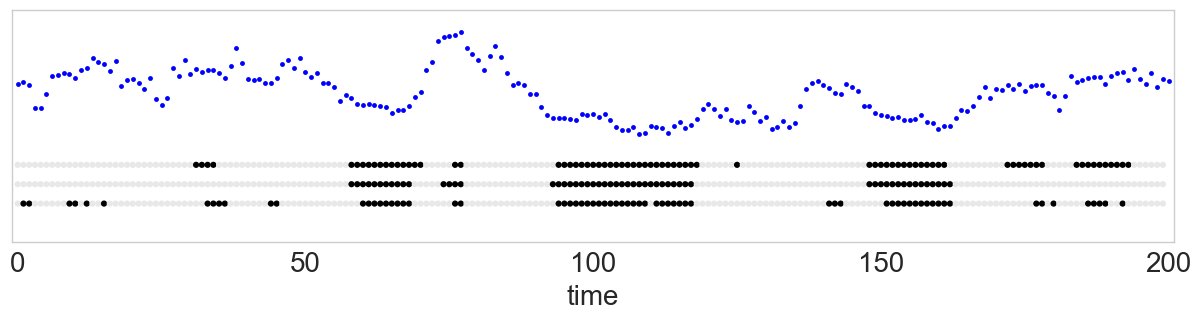
\includegraphics[width=\textwidth]{time_series_comparison.png}
\caption{An example of a generated time series from the SSSM model of Equation~\ref{eq:switching_state_space_results}. The $x$ axis represents time, and the $y$ axis shows the observations. Regime labels are shown as black and gray dots representing the two label options. True labels (top) are compared to the inferred labels from Algorithm~\ref{alg:constrained_alg} (middle) and the Gaussian merging (bottom).}
\label{fig:result_generated_time_series_with_labels}
\end{figure}

We ran Algorithm~\ref{alg:constrained_alg} to learn the switch points on this data, setting the number of regimes to nine. The percent agreement between the inferred regime labels and the known labels presents the accuracy for each algorithm for each time series. Figure~\ref{fig:result_generated_histograms} shows a histogram of the algorithm accuracy according to Algorithm~\ref{alg:constrained_alg} ($a$) and the baseline Gaussian merging ($b$). The bi-modal and long tailed distribution for the baseline approach demonstrates its susceptibility to local optima. When this algorithm converges toward the correct labeling, it finds a similar structure to that inferred by Algorithm~\ref{alg:constrained_alg}. However, if the initialization of the optimization (chosen randomly) is poor, this algorithm can easily result in labeling all of the data as belonging to one regime or the other. The mean accuracy of Algorithm~\ref{alg:constrained_alg} was 89\%, materially higher than the 66\% achieved by the Gaussian merging approach.

\begin{figure}
\centering
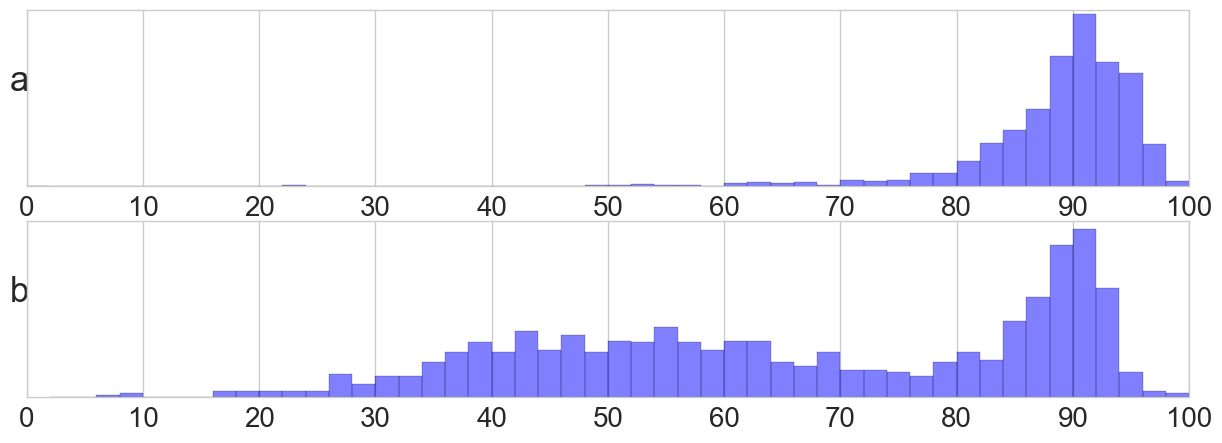
\includegraphics[width=\textwidth]{generated_results.png}
\caption{Histogram of the percent of correctly inferred labels for the observed output. The structured sampling Algorithm \ref{alg:constrained_alg} (a) learns the regime labels more accurately than the uninitialized Gaussian merging algorithm (b).}
\label{fig:result_generated_histograms}
\end{figure}

The superior performance of Algorithm~\ref{alg:constrained_alg} can be directly attributed to the switching behavior that is enforced by Assumptions 1 and 2, which was not assumed by the baseline model. Although Algorithm~\ref{alg:constrained_alg}'s model structure encourages the discovery of switches, the uniformly spaced initialization of labels should not be seen as an advantage as no prior knowledge of the actual switches is used in performing this step. The justification for enforcing the static number of switches is from Assumption 2 where the goal is to find more stable regimes and thus a lower frequency of switches between regimes. An implementation note is that although Algorithm~\ref{alg:constrained_alg} searches for $9$ regimes in the data, we know that only two are present. We therefore use a hierarchical structure to link the interleaving regimes which force the model to switch between the two regimes at successive switch points. The number of regimes for the Gaussian merging approach is set to two.

\section{Validation of Model Interpretability}

Algorithm~\ref{alg:constrained_alg} is aimed to assist teachers when leading their students through a review discussion of a particular simulation session. Thus we aim to validate that the inferred switch points are interpretable to a human seeking to understand the ``story'' of the simulation. The CW system provides a video representation of the log positions and the resulting water flow in the simulation. See Figure~\ref{fig:connected_worlds_graphic} for one frame from the video visualization that shows the biome positions, a distribution of logs on the floor of the simulation and the resulting flow of water at that time step. This video representation was presented to human validators to verify the change points that are found by Algorithm~\ref{alg:constrained_alg} (presented in Section \ref{sec:experiment1-empirical-validation}) and to verify the intelligibility of the automatically generated descriptions for the inferred periods (presented in Section \ref{sec:experiment2-empirical-validation}).

\subsection{Experiment 1}\label{sec:experiment1-empirical-validation}

We designed an experiment\footnote{Available at \url{http://essil-validation.s3-website-us-east-1.amazonaws.com/}} that asked evaluators to select one of three possible switch points between every pair of consecutive periods. Evaluators saw a composite of 1) the movie of the two periods; 2) a description of the dynamics of each of the two periods (e.g. ``water flows to the Desert and Plains'') and 3) a set of three possible switch points between the periods. The evaluator's task was to choose the switch point that best matched the change in dynamics between the two periods. One of the three switch points was that inferred by Algorithm~\ref{alg:constrained_alg}; the other two were random times sampled uniformly from the beginning of the first period to the end of the second period with the constraint that any two presented times cannot be within $10s$ of one another.

Evaluators worked with five sessions, each of which included $8$ to $12$ periods of system dynamics. Selecting the correct switch point is not a trivial task: it requires distinguishing between changes in the system that indicate different dynamic regimes and those that are noise within the same dynamic regime. We see an evaluator's ability to choose a switch point based on the movie and a description of the two contiguous periods as evidence that the inferred periods are potentially useful to a teacher who wants to guide students in constructing a causal description of their experience with the simulation.

\subsection{Experiment 1 Results}\label{sec:experiment1-empirical-validation-results}

Figure~\ref{fig:results_expert_validation} presents the results of the validation using four evaluators with knowledge of the CW domain. The five sessions are shown along the x-axis; the fraction of correctly selected switch points is shown by the bin heights. The dashed line represents a random baseline in which the selected switch probability corresponds to $\frac{1}{3}$. Under the null hypothesis, the performance of an evaluator would not be significantly different than the random baseline. The results indicate that the evaluators chose the switch point identified by Algorithm~\ref{alg:constrained_alg} significantly more often than the random baseline ($p < 1\times 10^{-4}$). This suggests that the inferred switch points were, indeed, interpretable to a large extent as meaningful changes in the state of the system. The differences in interpretability seen in Figure~\ref{fig:results_expert_validation} (e.g. Session 4 was more difficult to interpret than Session 3) can provide further guidance in how to support teachers and students in making sense of their experiences in CW.

\begin{figure}
\centering
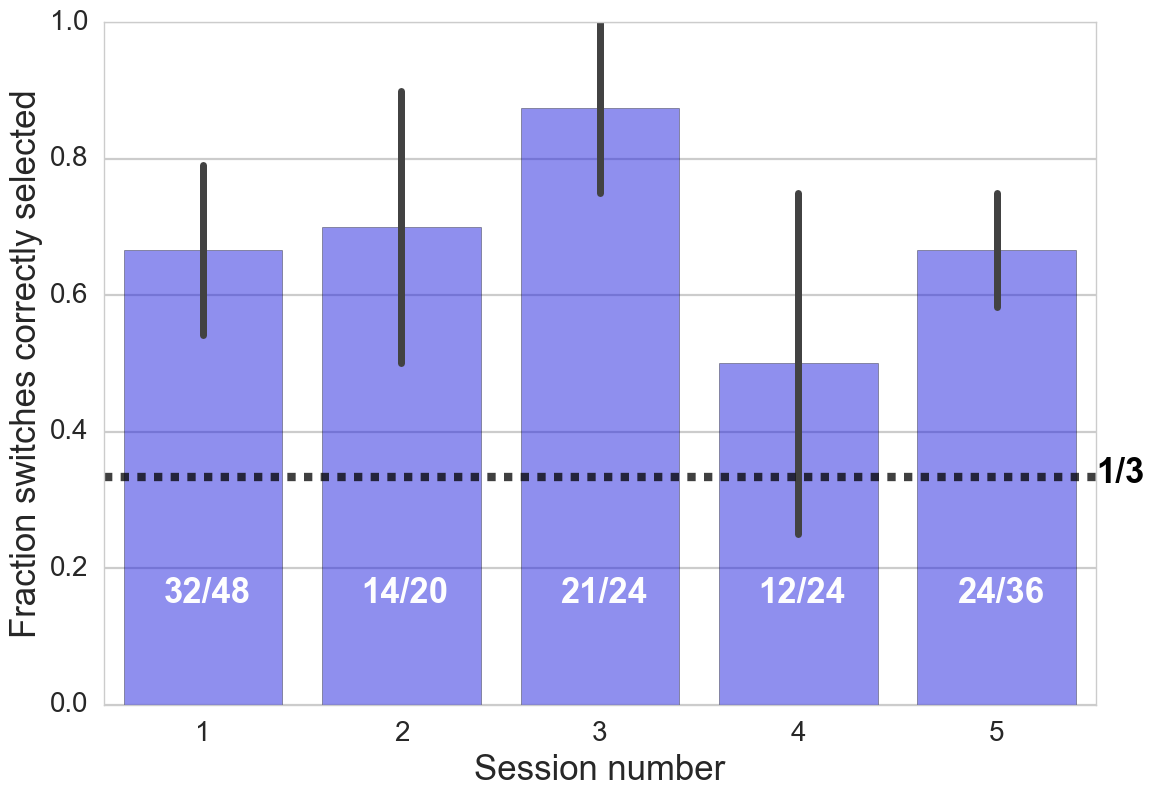
\includegraphics[width=10cm]{expert_validation_result.png}
\caption{Expert validation of five different test files from sessions with CW. The bar plot shows the fraction of correctly identified switches between automatically identified periods.}
\label{fig:results_expert_validation}
\end{figure}

\subsection{Experiment 2}\label{sec:experiment2-empirical-validation}

Experiment 2 aims to test the interpretability of the automatically generated regime descriptions when presented alongside the associated period clip from the video representation of the students' work. Validators are asked to choose one of three plausible descriptions for the dynamics that are displayed in the clip of the period. Experiment 2 further introduces a control condition where the change points in the time series are pre-defined and the descriptions are generated, conditioned on the pre-defined change points.

Figure~\ref{fig:user_experiment_overview} shows a screen-shot of the visualization\footnote{Available at \url{https://essil-validation.herokuapp.com/}} that the users are given. Label (1) shows the video clip; this clip is played for the duration of an inferred period. Label (2) indicates one of three descriptions that might be associated with the video clip. Validators are asked to watch the video and select the description that most accurately describes the dynamics in the video for the period. The dummy descriptions for each period are randomly generated.

\begin{sidewaysfigure}
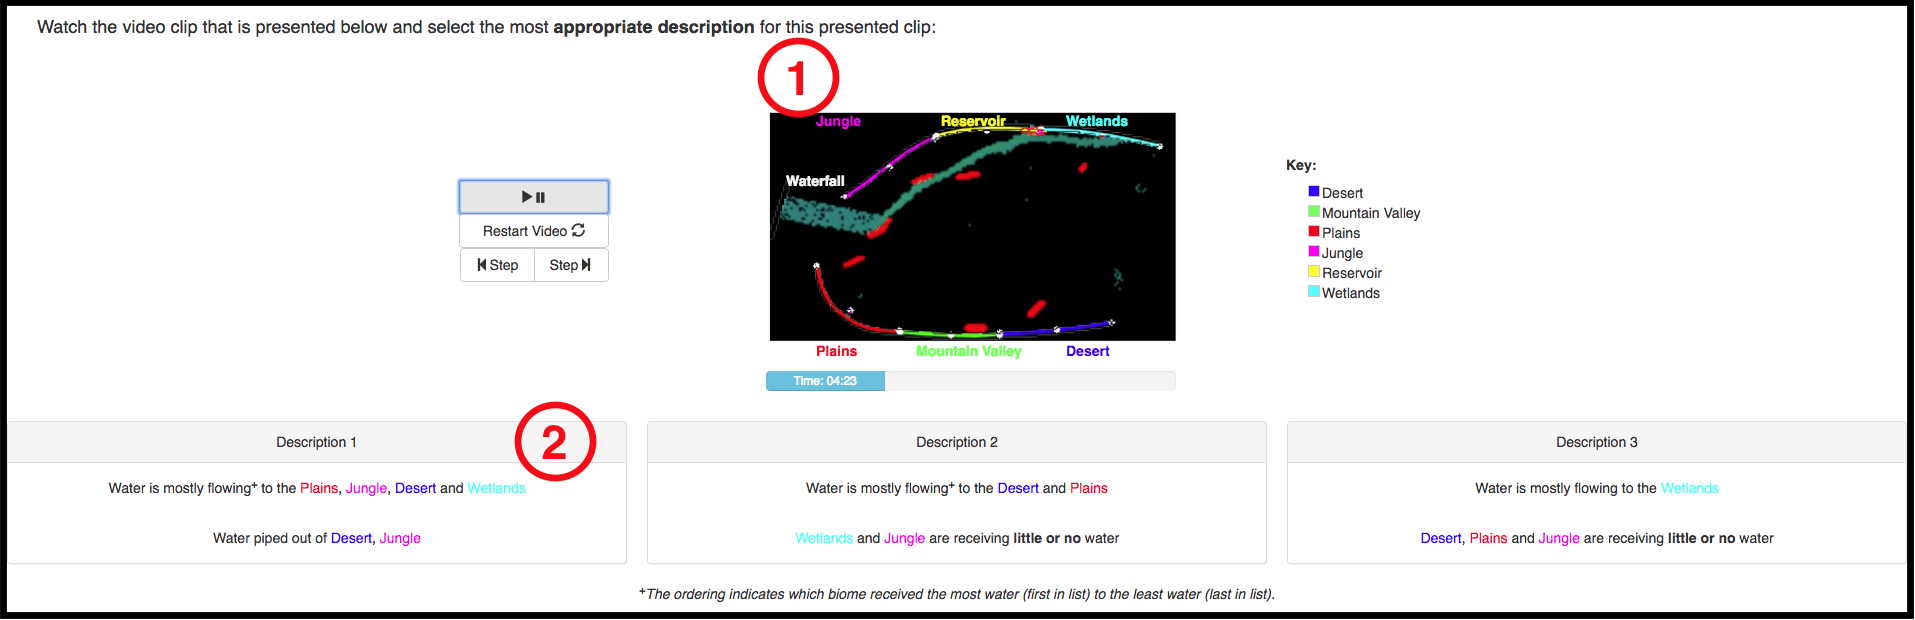
\includegraphics[width=\textwidth]{user_experiment_overview.png}
\caption{Screen-shot of the user interface designed to evaluate the interpretability of Algorithm~\ref{alg:constrained_alg}. The video representation at (1) is played for the duration of the period. Three plausible descriptions (of which (2) is one of these) are presented and the validator is asked to select the description that best describes the dynamics shown in the video. In this case, \textit{Description 3} is the correct solution.}
\label{fig:user_experiment_overview}
\end{sidewaysfigure}

The control condition in this experiment is to compare the algorithmically inferred period boundaries with boundaries that are uniformly spaced over the duration of the time series. We return to the hypothesis that deconstructing the time series into smaller periods will improve the period interpretability as the complexity of the period must decrease for shorter period lengths. Allowing Algorithm~\ref{alg:constrained_alg} to define the period boundaries should assist in finding periods that are more coherent for the associated descriptions. The algorithmically inferred periods should therefore be easier to identify than the periods that are defined uniformly across the time series.

The visualization (represented by the screen-shot in figure~\ref{fig:user_experiment_overview}) was presented to $40$ independent validators. Each participant had little or no prior knowledge about CW. A short tutorial of $14$ slides introduces the objective for validation and explains the key aspects of the video. The participants are shown $8$ randomly selected periods from the control and the test groups. The validators are required to watch the video associated with the period and select the description that most accurately describes the water dynamics. The results from Experiment 2 are given in Section~\ref{sec:experiment2-empirical-validation-results}.

\subsection{Experiment 2 Results}\label{sec:experiment2-empirical-validation-results}

$40$ validators independently labeled $296$ periods. The periods were generated from the same 5 session files that were presented in Section~\ref{sec:experiment1-empirical-validation}. The five files respectively had $12$,$8$,$8$,$8$ and $10$ inferred periods from Algorithm~\ref{alg:constrained_alg}. The control condition was implemented with a uniform period spacing with $8$ periods and again with $5$ periods in all $5$ test files. Figure~\ref{fig:experiment2_raw_results} shows the raw accuracy that was achieved for each file, under each algorithm. It can be seen that increasing the number of periods has a marked increase in the interpretability of the inferred description and video clip pairs. It is also interesting to note the same general structure of the bar plot as that seen in Figure~\ref{fig:results_expert_validation}, with file $3$ having the highest success rate and file $4$ having the lowest. The file appears to affect the interpretabilty of the periods in a similar manner for both experiments. This is intuitively correct as sessions where the system dynamics are more stable (possibly due to students executing fewer actions or having a simpler goal) might make for simpler and more easily understood descriptions. However, in cases where there are possibly many conflicting student agendas, the resulting dynamics might be complex and hard to interpret.

\begin{figure}
\centering
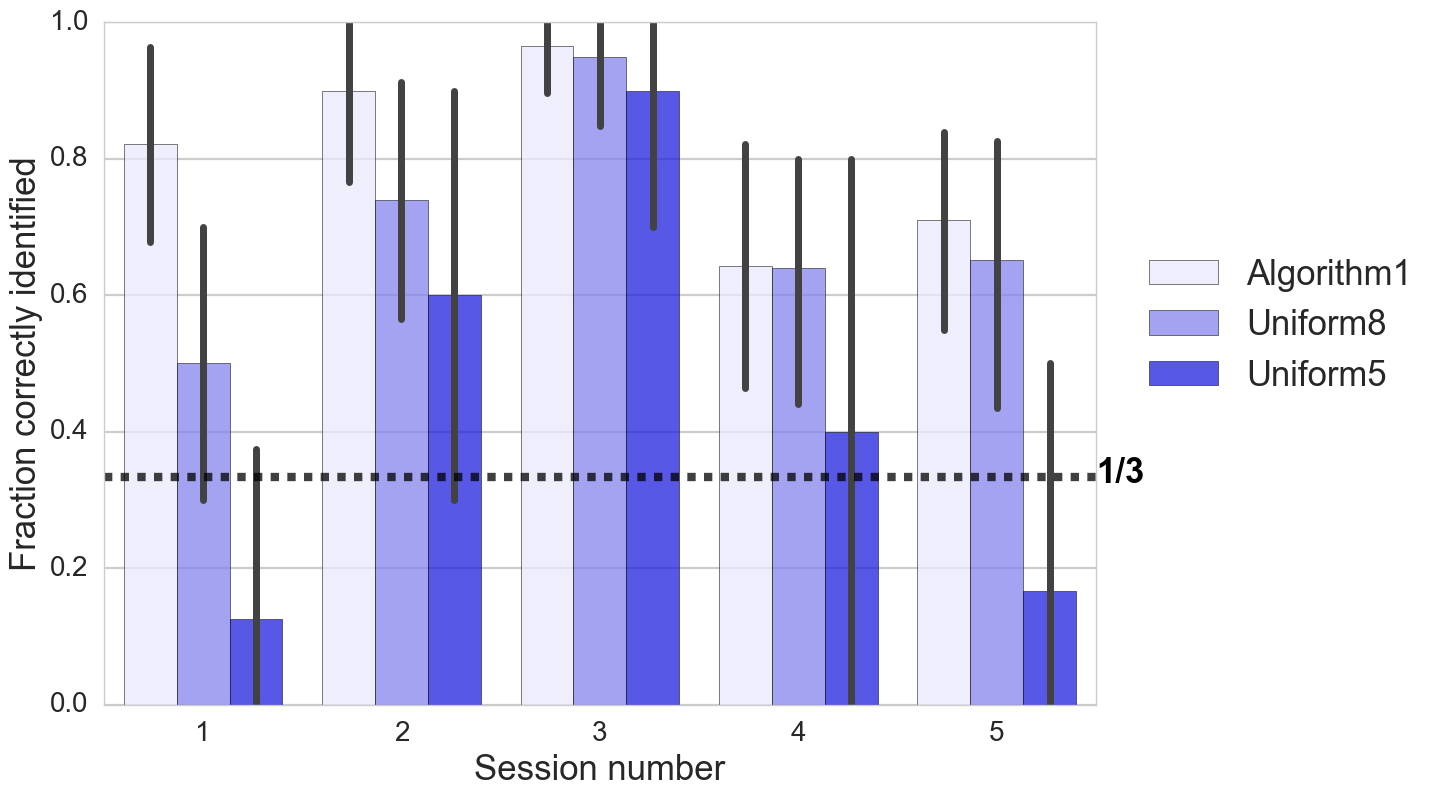
\includegraphics[width=12cm]{experiment2_raw_results.png}
\caption{Bar plot of the results from Experiment 2. There are 5 files that were tested. The fraction of correctly selected period descriptions from Algorithm~\ref{alg:constrained_alg} is compared to that from the control conditions. The control conditions include uniformly spaced periods for $8$ and $5$ periods respectively.}
\label{fig:experiment2_raw_results}
\end{figure}

Noting that the interpretability of the periods is file specific, we design a logistic regression analysis of the results. Specifically, a hierarchical logistic regression was conducted to determine the effect of the different algorithms on the probability that a validator successfully chooses the given algorithm's generated description. We compare the effects of seeing periods and descriptions from Algorithm~\ref{alg:constrained_alg} and the control with $8$ periods (Uniform8) to the baseline of the control with 5 periods (Uniform5).

The graphical model for the hierarchical logistic regression is presented in Figure~\ref{fig:hierarchical_logistic_regression}. $\mu_f$ refers to a file specific `ease of labeling'. The Algorithm~\ref{alg:constrained_alg} and Uniform8 `interpretability' effects are added to the file specific parameter. Period specific parameters are drawn from a normal prior distribution with mean defined by the file parameter and the effect of the algorithm used. Each period specific parameter $p_i$ represents the log-odds of a successful outcome in a Bernoulli trial. Note that the period specific parameters $p_i$ depend on the mean defined by the file and the algorithm that was used to generate the period. The variance around the file-algorithm mean is defined by the parameter $\sigma$, shared among all periods. $\sigma$ is an unknown model parameter and thus we place a weakly informative $\mathcal{N}(0,1)$ prior on this parameter. We conduct inference over the algorithm interpretability effect parameters ($\alpha_a$) and the period specific log-odds parameters (presented in Appendix~(TODO)).

\begin{figure}
\centering
\includegraphics[width=10cm]{hierarchical_logistic_regression.png}
\caption{Graphical model for the hierarchical logistic regression that is conducted to determine the interpretability effect of Algorithm~\ref{alg:constrained_alg} and Uniform8 over the base Uniform5 condition. The observed data $y$ corresponds to a Bernoulli trial where a description is selected to match a video clip or not. A given trial has a period specific probability of being chosen correctly $p_i$. $p_i$, in turn, depends on the file's ease of labeling and the algorithm effect. The $\alpha_a$ parameters represent the effect of the algorithm on the probability of correctly selecting the appropriate description. The periods depend on the file and algorithm means by a global variance parameter $\sigma$.}
\label{fig:hierarchical_logistic_regression}
\end{figure}

\begin{equation}\label{eq:generative_sampling_hierarchical_log}
  \begin{split}
    y_{i,k} &\mid p_i \sim Bern(logit^{-1}(p_i)) \\
    p_i &\mid \mu_f,\alpha_a,\sigma \sim \mathcal{N}(\mu_f + \mathbb{1}\{a\} \alpha_a, \sigma ) \\
    \mu_f &\sim \mathcal{N}(0,1) \\
    \sigma &\sim half\mathcal{N}(0,1)
  \end{split}
\end{equation}

The generative sampling distributions are given in Equation~\ref{eq:generative_sampling_hierarchical_log}. The inverse logit function is used to map the real valued log-odds parameter $p_i$ to a probability between $0$ and $1$. $\alpha_a$ refers to the algorithm specific interpretability effect, with $\alpha_1$, the parameter associated with using Algorithm~\ref{alg:constrained_alg} and $\alpha_2$, the parameter associated with using Uniform8 to generate the period. $\mathbb{1}\{a\}$ is the indicator that algorithm $a$ was used to produce the description and define the duration for period $i$.

The mean posterior value for $\alpha_1 = 2.03$ with a Bayesian $95\%$ posterior confidence interval of $[1.18, 2.96]$. The value is quoted in log-odds and corresponds approximately to being $\sim 8$ times more likely that a validator will select a period correctly under Algorithm~\ref{alg:constrained_alg} than under the baseline Uniform5. This is a highly significant result suggesting that Algorithm~\ref{alg:constrained_alg} improves on the baseline Uniform5 with 5 splits. The control group with 8 uniformly spaced periods has a posterior mean $\alpha_2 = 1.28$ (multiplicative effect of $\sim 4$ times more likely to select the period correctly over Uniform5) with a posterior confidence interval of $[0.43, 2.21]$. This too does not include $0$, the expected value for no discernible improvement, and therefore suggests that merely increasing the number of periods does help to make the periods more interpretable. However, Algorithm~\ref{alg:constrained_alg} can be compared to Uniform8 by evaluating the probability $P(\alpha_1 > \alpha_2)$. In other words, we are interested in the probability that Algorithm~\ref{alg:constrained_alg} is associated with a greater probability of choosing the generated description. This posterior probability is significant with a p-value of $p = 0.04$. The results suggest that the presented Algorithm~\ref{alg:constrained_alg} significantly improves the interpretability of the generated descriptions.

The structure of the inference executed in section~\ref{sec:experiment2-empirical-validation-results} allows us to consider the posterior probability for $p_i$ for each of the presented periods. This discussion is given in Appendix(TODO).%~\ref{}.




\chapter{Conclusion}\label{ch:4}
\section{Future Work}
There are two areas to be considered for future work. Firstly, Algorithm~\ref{alg:constrained_alg} assumes a known number of regimes. This is problematic in that sessions of different lengths or complexities would naturally have a different number of periods. It is not clear how to choose this number for a given session yet, as was seen in Section~\ref{sec:experiment2-empirical-validation}, it can have a major effect on the algorithm output. Bayesian non-parametrics presents a technique for remaining agnostic about the number of regimes to search for. Section~\ref{sec:non-parameteric} reviews related work in Bayesian non-parametrics for HMMs and we motivate why these models are promising for this domain. In Section~\ref{sec:class-assistive} we discuss the future work that builds on this thesis with the aim of working towards our original goal of presenting a tool that assists teachers when reviewing sessions from Connected Worlds.

\subsection{Bayesian Non-parametric Learning for the SSSM}\label{sec:non-parameteric}
\subsubsection{Introduction to Hierarchical Dirichlet Process}
The Dirichlet process (DP)~\citep{ferguson1973bayesian} defines a distribution over probability measures on a parameter space $\Theta$. It is parameterized by $G_0$, a base distribution, and $\alpha$, a concentration parameter. The DP consists of discrete atoms that are distributed on the base measure $G_0$ with mass that depends on $\alpha$.

\begin{equation}\label{eq:dirichlet_process}
  \begin{split}
    G \mid G_0, \alpha &= \sum\limits_{k=1}^{\infty} \beta_k \delta_{\theta_k} \\
    \theta_k \sim G_0
  \end{split}
\end{equation}

$\delta$ in equation~\ref{eq:dirichlet_process}, refers to the Kronecker delta function and represents the atoms of $G$ that are distributed according to $\theta_k \sim G_0$. The atoms have mass $\beta_k$, where $\beta \sim GEM(\alpha)$~\citep{neal2000markov}. Note that the Dirichlet process consists of infinitely many atoms; the term Bayesian non-parametrics stems from this countably infinite number of parameters. The DP can be used to model a countably infinite number of mixtures in a mixture model. Here each $\theta_k$ describes the parameters associated with mixture component $k$ and this component has a mixture weight given by $\beta_k$.

The Chinese Restaurant Process (CRP)~\citep{neal2000markov, gershman2012tutorial}, is an abstraction of the DP. It marginalizes over the probability associated with an atom and instead presents the DP in terms of the clusters that are formed. The CRP imagines a restaurant with an infinite number of tables, tables being the components in the mixture model. Customers (data) arrive at the restaurant and choose a table with probability proportional to the number of customers already at that table, or choose a new table with probability proportional to $\alpha$. As more customers enter the restaurant, more tables are chosen with:
\begin{equation}
  E[N_t] = \alpha \log(N_c)
\end{equation}
$N_t$ and $N_c$ refer to the number of tables and customers respectively~\citep{gershman2012tutorial}. The number of components is random and grows as new data are observed. It is important to understand that while conceptually, and for the generative model, there are an infinite number of components, in practice a finite dataset exhibits a finite number of clusters (only a finite number of tables can have customers seated at them)~\citep{blei2006variational}.

The hierarchical Dirichlet process (HDP) extends equation~\ref{eq:dirichlet_process} by placing a Dirichlet process prior on many group specific Dirichlet processes~\citep{teh2005sharing}. The associated abstraction is the Chinese Restaurant Franchise (CRF) where restaurants may have menus that offer the same dish, but may also have dishes that are restaurant specific. This allows restaurants to assign different mass to table clusters where the customers still have the same dish. Now customers choose a restaurant in a franchise and choose a dish from the restaurant of choice. The HDP draws $G_0$ from a Dirichlet process $DP(\gamma, H)$, and it draws group (restaurant) specific distributions $G_j \sim DP(\alpha, G_0)$. The base measure $G_0$ acts as the expected value for encoding the frequency of each global, shared parameter~\citep{fox2007hierarchical}.

\begin{equation}
  E[G_j \mid G_0] = G_0
\end{equation}

\subsubsection{Hierarchical Dirichlet Process for Hidden Markov Models}
We may wish to use the HDP as the clustering prior to infer the parameters and transition probabilities in a HMM. We assume an unknown number of regimes and thus model this with a DP prior. Simply using a DP prior is insufficient for modeling HMM dynamics as the DP would place a static probability on observing the next state $X_t \mid X_{t-1}$ for all possible $X_{t-1}$ which is clearly not the case for the HMM. The transition to state $X_t$ from $X_{t-1}$ must depend on state specific probabilities $\pi_{X_{t-1}}$ and not some global partition prior $\pi$. The HMM therefore involves a set of mixture models that each depend on a specific state. The state indexes a row of the transition matrix, where the probabilities in this row correspond to the mixing proportions for the choice of the next state. We therefore encode this state (regime) dependent transition by using the HDP which still encourages shared structure between the individual transitions. Now each regime $m$ might have its specific transition probabilities $\pi_m$ but the different regimes might share the affinity to transition to certain `dominant' regimes.

\cite{fox2009nonparametric, fox2007hierarchical} discuss problems with the HDP approach. The HDP-HMM inadequately models the temporal persistence of states. Each state is allowed to have a unique transition mixture, with mass shared among states for certain transitions that are more probable. However, it is impossible to encourage self transitions with simply the base hierarchical parameter $H$. The result is that the HDP-HMM exhibits a rapid inferred switching from one state to the next~\citep{fox2007hierarchical}. Rather, if we introduce a higher probability of a self transition, we encourage the HMM to have an affinity for remaining in any given regime for a greater length of time. This directly ties to Assumption 2 in Section~\ref{sec:inference_for_sssm}.

The adjustment to the HDP-HMM that \cite{fox2009nonparametric,fox2007hierarchical} propose is to add a self-transition affinity parameter $\kappa$. The resulting model is termed the sticky hierarchical Dirichlet process for hidden Markov models (sticky HDP HMM). Inference is performed using a modified Gibbs sampler for the HDP~\citep{teh2005sharing}. This model presents an attractive alternative to Algorithm~\ref{alg:constrained_alg} as the number of regimes is not pre-defined and more importantly, the model specification allows the growth of the number of regimes with the length and/or complexity of the data. This captures the intuitive reality of the simulation more accurately in that we would want more regimes to describe longer and more complex sessions.

An avenue for the extension of the \cite{fox2009nonparametric} model is to encourage the linear growth of the number of regimes with the length of a given session. The Pitman-Yor process~\citep{pitman1997two} extends the DP for linear growth of clusters (not logarithmic as presented above). \cite{blunsom2011hierarchical} have applied this concept to develop the hierarchical Pitman-Yor process HMM. It seems natural to extend these models to include the regime affinity parameter $\kappa$ from \cite{fox2007hierarchical,fox2009nonparametric}.

\subsection{The SSSM as an Assistive Classroom Tool}\label{sec:class-assistive}
With the introduction of rich and complex learning environments, we should remain aware that these simulations pose challenges for teachers who wish to structure learning around a class's session. These teachers may require additional tools to assist them with the domain specific challenges that arise when designing lesson plans around sessions with these simulations. In Section~\ref{sec:need_for_assistive_tech}, we discussed how it is hard for a participant or observer to track the state of the CW simulation. It is therefore also challenging to identify the salient learning opportunities that arise from the students' interactions with the simulation. In addition to this, standard evaluation metrics might not be available for activities engendered by these complex simulations. The investigation of how to integrate these tools into the class is therefore of paramount importance.

Section~\ref{sec:user_evaluation} presents a study that demonstrates how the SSSM is used to decompose a large session from CW into small periods that individually are interpretable. This thesis has focused mainly on the time series data itself and has presented techniques for modeling the effects of students' actions on the system state. Future work will investigate the application of these models for producing an assistive system for implementation in the classroom. An investigation into the techniques for presenting a meaningful, holistic picture of the session remains for future studies.

The design of classroom assistive tools should focus on what information they present to the students as well as how they present the information. We propose two principles for choosing information that is relevant to present to students and teachers:
\begin{itemize}
  \item \textbf{Personal salience}: includes scenarios from the simulation experience that are likely to be memorable for the students.
  \item \textbf{Explanatory coherence}: includes a subset of the simulation’s causal chains that enables students’ discussion of an aspect of the underlying explanatory model.
\end{itemize}

The work in this thesis has focused solely on the \textit{explanatory coherence} topics. A full assistive model will not only include information that describes system dynamics and changes to the system state, but it will also highlight key elements from the simulation that will be important to the individual students. The proposed future work involves designing, implementing and testing this classroom tool.

Another exciting avenue for future research involves exploring the trade-off that is made between the predictive power of a model and the explanatory coherence that the model achieves. \cite{wu2017beyond} have suggested a method for regularizing deep learning models to facilitate people's understanding of their predictions. This is an important balance to review and one that we intend to consider in educational settings.

\section{Conclusion}

This thesis has made three contributions. Firstly, we have recognized that complex exploratory learning environments might require assistive tools to help teachers and students review meaningful information from a given interaction session. This novel research has studied the possibilities for extracting information from the log files of an exploratory learning environment. We used the Connected World simulation as a test case and represented the logs as a time series. It was our hypothesis that a time series can be decomposed into shorter periods that are individually more interpretable and manageable than the session as a whole.

Secondly, we have applied switching state space models to the task of decomposing the time series into shorter and individually coherent periods. Our work has built upon previous time series analysis tools and presents an algorithm for learning the change points and regime parameters that are associated with the switching state space model. We have further conducted a survey of possible future work in Bayesian non-parameterics for allowing the data to influence the number of regimes that are inferred in a given session. A flexible number of regimes is especially appealing for a setting such as Connected Worlds where the sessions vary dramatically in length and complexity.

Lastly, we have designed two user-based experiments that test the understandibility and change point relevance of the model output. The human interpretability of the model was the ultimate goal of this investigation. However, evaluating the different aspects of the model (`learning' vs `quantification') was a challenging task. Our experiments suggest that the model not only finds a good representation of the periods that might be present in Connected Worlds, but that it also summarizes each period (of about 30 seconds) into a brief two to three lines of text. The generated text captures much of the dynamics of an associated video representation of the period. Between the two studies, we show that it is possible to simplify a complex time series into periods of activity that are human interpretable.

We have left the design and implementation of a classroom tool as future work. This tool should aim to interactively support teachers and students for post session reviews. This work presents exciting new possibilities for classroom artificial intelligence tools that can support learning in these rich and immersive exploration environments.


%%%%%%%%%%%%%%%% BACK MATTER %%%%%%%%%%%%%%%%

% Put appendices, bibliography, and supplemental materials here

% The bibliography may be single spaced within each entry, but must be
% double-spaced between each entry. Most bibliography styles leave space between
% entries, so that shouldn't be a problem.
\begin{singlespacing}
  % I like "References" better than "Bibliography"
  \renewcommand{\bibname}{References}

  % Any bibliohgraphy style that leaves space between entries is fine
  \bibliographystyle{ecca}
  \bibliography{references}
\end{singlespacing}

% Appendices from all chapters should go at the end
\begin{appendices}

\chapter{Plant and Animal Relations}\label{cha:appendix2}
For completeness, we have included a map to highlight the relationships between the plants and animals in Connected Worlds. Students plant trees and observe the arrival of animals that use the trees to support their habitat. Mimicking a real-world scenario, the fauna for a biome depend on the flora, and the flora are unique for a specific biome. Larger and higher level plants require the presence of smaller and lower level plants. Figure~\ref{fig:system_overview_plant_animal} shows a schematic that displays the plant and animal relations of Connected Worlds.

\begin{figure}
\centering
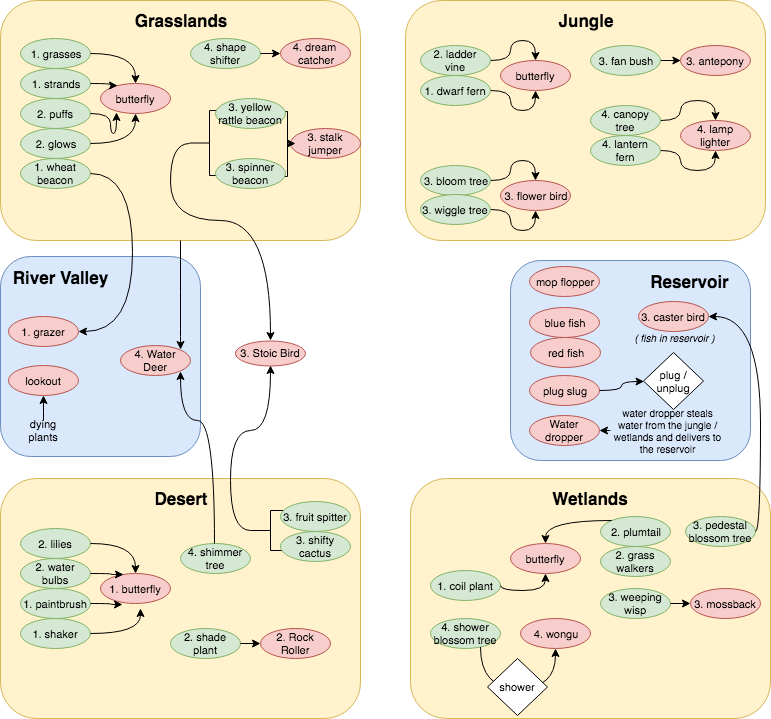
\includegraphics[width=\textwidth]{system_overview_plant_animal.png}
\caption{Map of the relationships between plants, animals and biomes in the CW environment. The biomes are shown in yellow. The blue boxes correspond to areas of the simulation that do support animals but do not have plants that grow there. The fauna-flora specific relations can clearly be seen by the arrows that link the plants (green ovals) and animals (red ovals). The plants and animals are endemic to their biome.}
\label{fig:system_overview_plant_animal}
\end{figure}



\chapter{Posterior Probability of Correct Period Selection}\label{cha:appendix1}
\begin{figure}
\centering
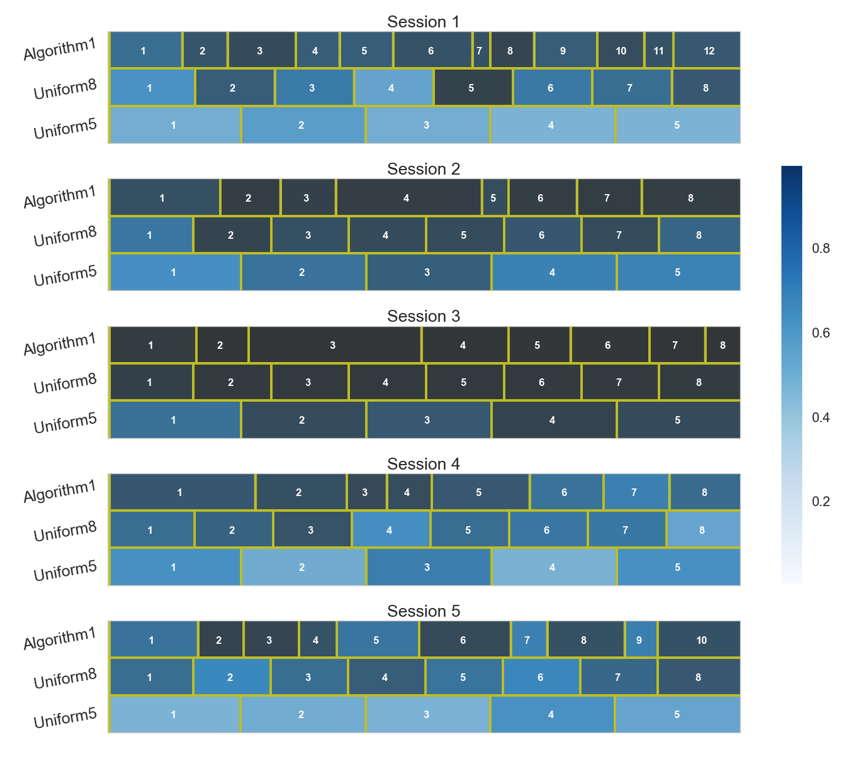
\includegraphics[width=\textwidth]{posterior_pvalues.png}
\caption{Diagram to represent the periods that are inferred by Algorithm 1 in comparison to those defined by Uniform5 and Uniform8. The vertical yellow lines denote the period boundaries and the color of the period presents the posterior probability that an external validator will select the text description that is generated by the algorithm. Dark colors correspond to high probability for being selected and light colors correspond to a low probability.}
\label{fig:posterior_pvalues}
\end{figure}

Figure~\ref{fig:posterior_pvalues} presents a visualization of the period boundaries for the $5$ sessions that were studied in the text. The x-axis corresponds to time and the y-axis shows the algorithm that was used to generate the boundaries. The vertical yellow lines indicate the inferred period boundaries; a period exists between two yellow boundaries. The periods are labeled sequentially for reference in this discussion. Finally, the color of the period indicates the posterior probability that a human validator will select the algorithmically generated description for that period. Light blue corresponds to a low probability of the algorithmic description being correctly chosen and dark blue or black corresponds to a high probability.

In general we note that the Algorithm 1 periods are darker than the periods of Uniform8; the Uniform8 periods are darker than the periods for Uniform5. We also note that when the period boundaries line up entirely (between different algorithms), the period colors tend to be very similar (refer to \textit{Session 1, Algorithm 1, period 12} and \textit{Session 1, Uniform8, period 8} for one such example). The file difficulty variability is seen with Session 3 being the darkest (easiest) and Sessions 4 and 5 being the lightest on average (i.e., for these two sessions, it was the most difficult to select the algorithm's generated description).

It is interesting to investigate some specific aspects of this visualization. Starting with Session 1, Algorithm~1 has a slightly darker period 1 than the other algorithms. Uniform8 and Algorithm~1 both present the description that ``Water is mostly flowing to the Wetlands, Jungle and Plains''. Uniform5 describes the longer period as water mostly flowing to the ``Jungle, Wetlands and Plains'' and so these are all similar. The dummy choices are reasonable in all three cases with one example being: ``Water is mostly flowing to the Plains, Jungle and Wetlands''. At time $t=44s$, the end boundary for Algorithm~1, period~1, the students position the logs to direct a substantial amount of water to the Jungle and to the Plains. Algorithm~1 correctly detected this change and defined a new period 2. In the other algorithms, as period 1 was extended into this dominant Jungle/Plains dynamic, the descriptions became more difficult to choose from (hence the lowest probability for a successful choice is seen in Uniform5). Figure~\ref{fig:test} shows four snapshots around the $44s$ change point where after $44s$, the water mainly flows to the Jungle and the Plains. It qualitatively seems natural to have a change point at this time.

\begin{figure}
\centering
\begin{subfigure}{.24\textwidth}
  \centering
  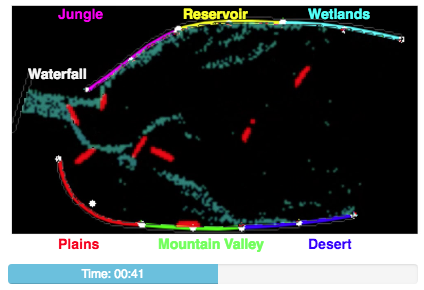
\includegraphics[width=\linewidth]{mov-im1}
  \caption{frame 1 (41s)}
\end{subfigure}%
\begin{subfigure}{.24\textwidth}
  \centering
  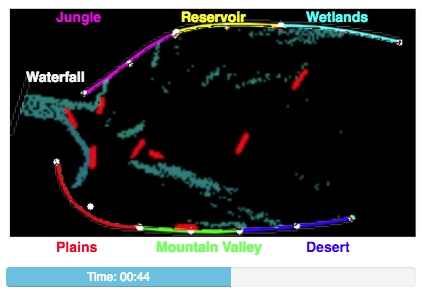
\includegraphics[width=\linewidth]{mov-im2}
  \caption{frame 2 (44s)}
\end{subfigure}
\begin{subfigure}{.24\textwidth}
  \centering
  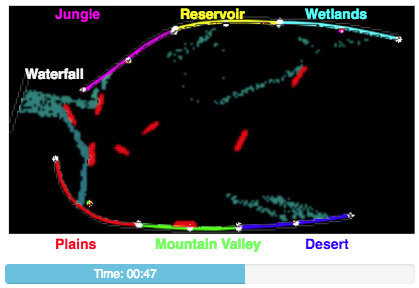
\includegraphics[width=\linewidth]{mov-im3}
  \caption{frame 3 (47s)}
\end{subfigure}
\begin{subfigure}{.24\textwidth}
  \centering
  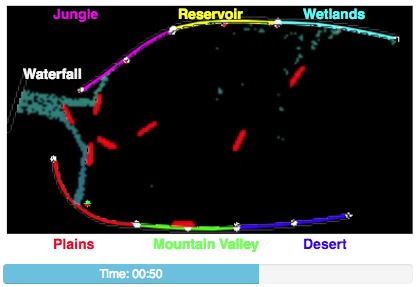
\includegraphics[width=\linewidth]{mov-im4}
  \caption{frame 4 (50s)}
\end{subfigure}
\caption{Sequence of $4$ snapshots from the video given to validators (each frame is 3 seconds apart). The logs are moved in frames 1 and 2 such that the water is mostly flowing to the Plains and Jungle in frames 3 and 4 and afterwards.}
\label{fig:test}
\end{figure}

Session 5, Algorithm 1, has light periods $7$ and $9$ interspersed by darker periods. For both of these periods, the Algorithm 1 description is misleading. The ordering of the parameters conveys a hierarchical structure to the message that is being conveyed. This is not always correct. In both of these cases, the parameters were actually similar in magnitude and thus the strict ordering of the description may have been misleading. In Section~\ref{sec:class-assistive}, we discuss how future work will entail correctly compiling the available information to design an assistive aid for teachers. Making decisions regarding how the data are presented will certainly from an important aspect of this work.

A final point that can be made from this session is that the rain events of the system are not identified well by the algorithm and can also lead to misleading descriptions that are generated. It remains a challenge to find a robust way for dealing with rain events. The simplest recommendation is to add these events to the log files that are stored as part of the output from CW.



\end{appendices}


\end{document}
